\documentclass[10.5pt,notitlepage]{article}
\usepackage[utf8]{inputenc}
\usepackage{amsthm}
\usepackage{amsmath}
\usepackage{amsfonts}
\usepackage{mathtools}
\usepackage{amsmath,amssymb}       
\usepackage{enumitem}   
\usepackage{enumerate}
\usepackage{verbatim} 
\usepackage{bbm}
\usepackage{hyperref}
\usepackage{booktabs}
\renewcommand{\qedsymbol}{$\blacksquare$}
\usepackage{makecell}
\usepackage[spanish]{babel}
\decimalpoint
\usepackage[letterpaper]{geometry}
\usepackage{mathrsfs}
\newenvironment{solucion}
  {\begin{proof}[Solución]}
  {\end{proof}}
\pagestyle{plain}
\usepackage{pdflscape}
\usepackage[table, dvipsnames]{xcolor}
\usepackage{longtable}
\usepackage{tikz}
\def\checkmark{\tikz\fill[scale=0.4](0,.35) -- (.25,0) -- (1,.7) -- (.25,.15) -- cycle;} 
\usepackage[bottom]{footmisc}
\usepackage{hyperref}
\usepackage{float}
\usepackage[utf8]{inputenc}
\usepackage{bbm}
\usepackage{placeins}
\newcommand{\pp}{\mathbb{P}}
\newcommand{\BB}{\mathcal{B}}
\newcommand{\RR}{\mathbb{R}}
\newcommand{\FF}{\mathcal{F}}
\newcommand{\CC}{\mathcal{C}}
\newcommand{\oo}{\varnothing}
\newcommand{\ee}{\varepsilon}
\newcommand{\NN}{\mathbb{N}}
\newcommand{\PP}{\mathcal{P}}
\newcommand{\LL}{\mathrm{L}}
\newcommand{\XX}{\mathbf{X}}
\newcommand{\xx}{\mathbf{x}}
\DeclareMathOperator{\Tr}{Tr}
\newcommand{\abs}[1]{\left\lvert #1 \right\rvert}
\newcommand{\norm}[1]{\left\| #1 \right\|}
\newcommand{\inner}[1]{\left\langle #1 \right\rangle}
\newcommand{\corch}[1]{\left[ #1 \right]}
\newcommand{\kis}[1]{\left\{ #1 \right\}}
\newcommand{\pare}[1]{\left( #1 \right)}

\theoremstyle{plain}

\newtheorem{thm}{Teorema}[section] % reset theorem numbering for each chapter
\newtheorem{defn}[thm]{Definición} % definition numbers are dependent on theorem numbers
\newtheorem{lem}[thm]{Lema} % same for example numbers
\newtheorem{remarkex}{Observación}
\newenvironment{rem}
  {\pushQED{\qed}\renewcommand{\qedsymbol}{$\triangle$}\remarkex}
  {\popQED\endremarkex}

\usepackage{geometry}
\usepackage{mathtools}
\usepackage{enumitem}
\usepackage{framed}
\usepackage{amsthm}
\usepackage{thmtools}
\usepackage{etoolbox}
\usepackage{fancybox}

\newenvironment{myleftbar}{%
\def\FrameCommand{\hspace{0.6em}\vrule width 2pt\hspace{0.6em}}%
\MakeFramed{\advance\hsize-\width \FrameRestore}}%
{\endMakeFramed}
\declaretheoremstyle[
spaceabove=6pt,
spacebelow=6pt
headfont=\normalfont\bfseries,
headpunct={} ,
headformat={\cornersize*{2pt}\ovalbox{\NAME~\NUMBER\ifstrequal{\NOTE}{}{\relax}{\NOTE}:}},
bodyfont=\normalfont,
]{exobreak}

\declaretheorem[style=exobreak, name=Ejercicio,%
postheadhook=\leavevmode\myleftbar, %
prefoothook = \endmyleftbar]{exo}
\usepackage{graphicx}
\graphicspath{ {images/} }
\title{Tarea 6: Modelos Estadísticos I.}

\author{Rojas Gutiérrez Rodolfo Emmanuel}

\date{\today}
\begin{document}

\maketitle

\begin{rem}
Para todos los modelos considerados aquí se supondrá que sus términos de error cumplen los supuestos usuales del modelo de regresión lineal, además para algunos resultados será de utilidad agregar el supuesto de normalidad de dichos términos de error.
\end{rem}
\setcounter{exo}{0}
\begin{exo}[Análisis de servicio hospitalario.] En la tabla \ref{tab:1} se muestran datos relacionados con las necesidades para el trabajo hospitalario provenientes de una muestra de \(17\) hospitales, de un sistema hospitalario determinado. La variable \(V1\) representa la carga promedio diaria de pacientes, \(V2\) denota el número mensual de rayos \(X\), \(V3\) denota el número de días cama de ocupación mensual, \(V4\) denota la población elegible en el área (dividida por 1000), \(V5\) denota la longitud promedio de permanencia de los pacientes, en días. La variable respuesta \(W\) es el número de horas de trabajo durante el mes. Hacer lo siguiente: 
\begin{itemize}
    \item[a)] Grafique los diagramas de dispersión de la variable respuesta con cada una de las variables independientes y también evalué los coeficientes de correlación entre la variable respuesta y cada una de las cinco variables regresoras. Comente los resultados de este inciso.
    \item[b)] ¿Que evidencia hay de la presencia de multicolinealidad en los datos de este problema? Haga los cálculos necesarios para la detección de la multicolinealidad.
    \item[c)] Calcule los factores de inflación de la varianza \(VIF\) para las cinco variables regresoras y deles una interpretación.
    \item[d)] Discuta la posibilidad de obtener modelos de regresión donde el impacto
de la multicolinealidad sea menor que en el modelo completo original con
las cinco variables regresoras.
    \item[e)] Proponga un modelo de regresión en el que la multicolinealidad es menor que en el modelo original.
\end{itemize}
\end{exo}
 \begin{table}[htbp]
        \caption{Datos de necesidades del trabajo en un sistema hospitalario determinado.}
        \centering\begin{tabular}{@{}l@{\hskip 0.3in}r@{\hskip 0.3in}r@{\hskip 0.3in}r@{\hskip 0.3in}r@{\hskip 0.3in}r@{}}
            \toprule
            $V1$ & $V2$ & $V3$ & $V4$ &\(V5\) &\(W\)\\
            \midrule
 15.57  &  2463 &     472.82&    18  &    4.45 &    556.52\\
 44.02  &  2048&   1339.75 &   9.5   & 6.92    & 696.82\\
 20.42  &  3940 &     620.25&    12.8&    4.28&    1033.15\\
 18.74  &  6505 &     568.33&    36.7 &   3.9   &  1603.62\\
 49.2   &  5723 &    1497.6 &    35.7&    5.5  &   1611.37\\
 44.92  & 11520 &    1365.83&    24  &    4.6    & 1613.27\\
 55.48  &  5779 &    1687   &    43.3&    5.62 &   1854.17\\
 59.28  &  5969 &    1639.92&    46.7&    5.15   & 2160.55\\
 94.39  &  8461 &    2872.33&    78.7&    6.18 &   2305.58\\
128.02  & 20106 &    3655.08&   180.5&    6.15   & 3503.93\\
 96     & 13313 &    2912   &    60.9&    5.88 &   3571.89\\
131.42  & 10771 &    3921   &   103.7&    4.88   & 3741.4\\
127.21  & 15543 &    3865.67&   126.8&    5.5 &    4026.52\\
252.9   & 36194 &    7684.1 &   157.7&    7     & 10343.81\\
409.2  &  34703 &   12446.33&   169.4&   10.78&   11732.17\\
463.7  &  39204 &    14098.4&   331.4&    7.05  & 15414.94\\
510.22 &  86533 &    15524  &   371.6&    6.35 &  18854.45\\
            \bottomrule
        \end{tabular}
        \label{tab:1}
\end{table}
\begin{solucion}
\textbf{a)} En la figura \ref{fig:1} se dejan las gráficas de dispersión solicitadas, en cada una de estás gráficas se puede ver un modelo de regresión lineal que ocupa en cada caso a una y solo una de las variables independientes \(V1, \hdots, V2\) para explicar a la variable respuesta \(W\), es importante destacar que tanto el modelo que tiene por variable explicativa a \(V1\) como el que tiene por variable explicativa a \(V3\), parecen ser bastante razonables para explicar a la variable respuesta \(W\) ya que presentan\footnote{Al menos visualmente.} una variabilidad aceptable en sus bandas de confianza y predicción, aquí uno podría pensar erróneamente en usar ambas variables como predictores para 'mejorar' estos modelos, o incluso usar todas las variables independientes, pero habrá que analizar la existencia de multicolinealidad entre ellas para determinar cuales podrían realmente aportar más a un modelo que busque explicar a \(W\), por otro lado las correlaciones solicitadas se encuentran a continuación, las mismas no agregan mucho más al análisis previamente mencionado.
\begin{table}[H]
        \centering
        \begin{tabular}{@{}l@{\hskip 0.3in}r@{\hskip 0.3in}r@{\hskip 0.3in}r@{\hskip 0.3in}r@{}}
            \toprule
            \(Cor(V1,W)\)& \(Cor(V2,W)\) & \(Cor(V3,W)\)& \(Cor(V4,W)\)& \(Cor(V5,W)\) \\
            \midrule
               0.986 &0.945 &0.986& 0.940& 0.579 \\  
            \bottomrule
        \end{tabular}
        \caption{Correlaciones de las variables independientes con la variable respuesta.}
\end{table}

Como primer paso para detectar problemas de multicolinealidad entre las variables independientes, se pensó que resultaría de gran utilidad realizar gráficas de dispersión para las mismas, por ende, se puede observar en las figuras \ref{fig:2}-\ref{fig:5} dichas gráficas, además, se agregó nuevamente una recta de regresión lineal e intervalos de confianza y predicción al \(95\%\) en cada caso a modo de indicador de la relación lineal existente entre las variables independientes. Se observa que en la mayoría de los casos pareciera existir colinealidad cuando menos moderada, sin embargo, la variable \(V5\) aparenta ser la que tiene la colinealidad más débil entre las diversas variables independientes, esto porque en la mayoría de los gráficos de dispersión los intervalos de confianza y predicción parecen abrirse mucho más que en los otros casos, indicando que hay gran variabilidad que no es explicada por ninguna de las otras variables independientes por separado. \\
\begin{figure}[htb]
 \centering
 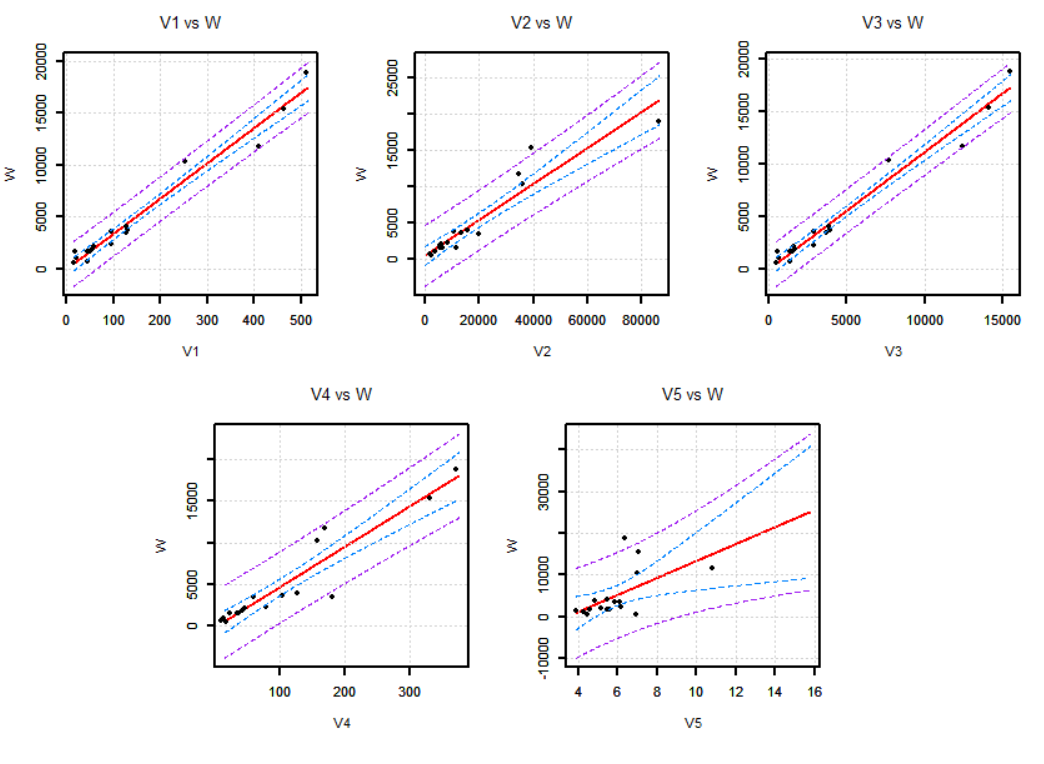
\includegraphics[scale = 0.65]{Imagen1Ej1T6.png}
 \caption{Gráficos de dispersión de cada una de las variables independientes \(\kis{V1,\hdots,V5}\) contra la variable respuesta \(W\). Se deja recta de regresión lineal (recta roja) e intervalos de confianza al \(95\%\) (rectas azules) y predicción al \(95\%\) confianza (rectas purpuras).}
\label{fig:1}
\end{figure}
\begin{figure}[htb]
 \centering
 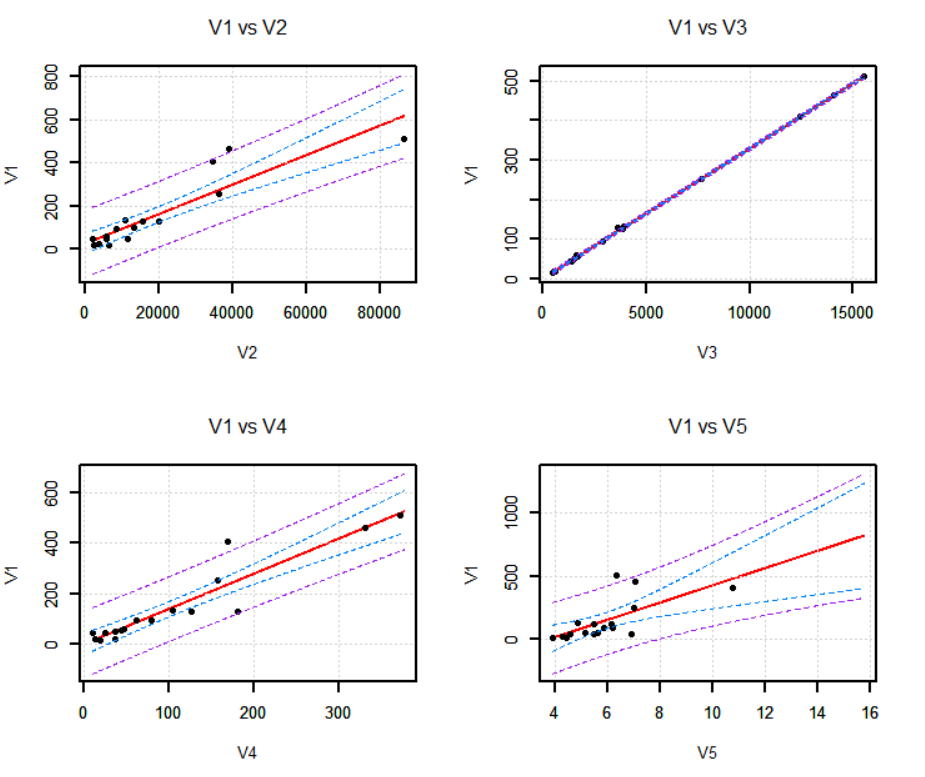
\includegraphics[scale = 0.65]{Imagen2Ej1T6.png}
 \caption{Gráficos de dispersión de las variables independientes \(\kis{V2,V3,V4,V5}\) contra la variable independiente \(V1\). Se deja recta de regresión lineal (recta roja) e intervalos de confianza al \(95\%\) (rectas azules) y predicción al \(95\%\) confianza (rectas purpuras).}
\label{fig:2}
\end{figure}
\begin{figure}[htb]
 \centering
 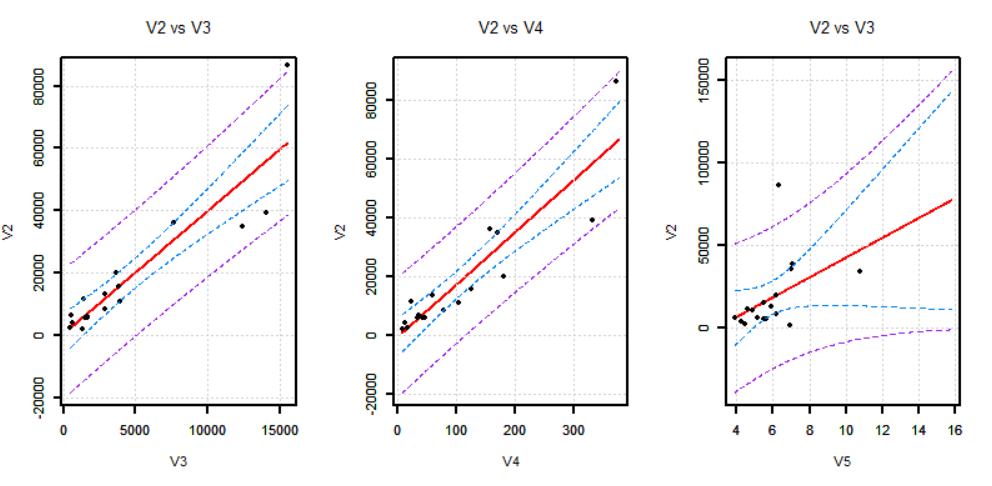
\includegraphics[scale = 0.65]{Imagen3Ej1T6.png}
 \caption{Gráficos de dispersión de las variables independientes \(\kis{V3,V4,V5}\) contra la variable independiente \(V2\). Se deja recta de regresión lineal (recta roja) e intervalos de confianza al \(95\%\) (rectas azules) y predicción al \(95\%\) confianza (rectas purpuras).}
\label{fig:3}
\end{figure}
\begin{figure}[htb]
 \centering
 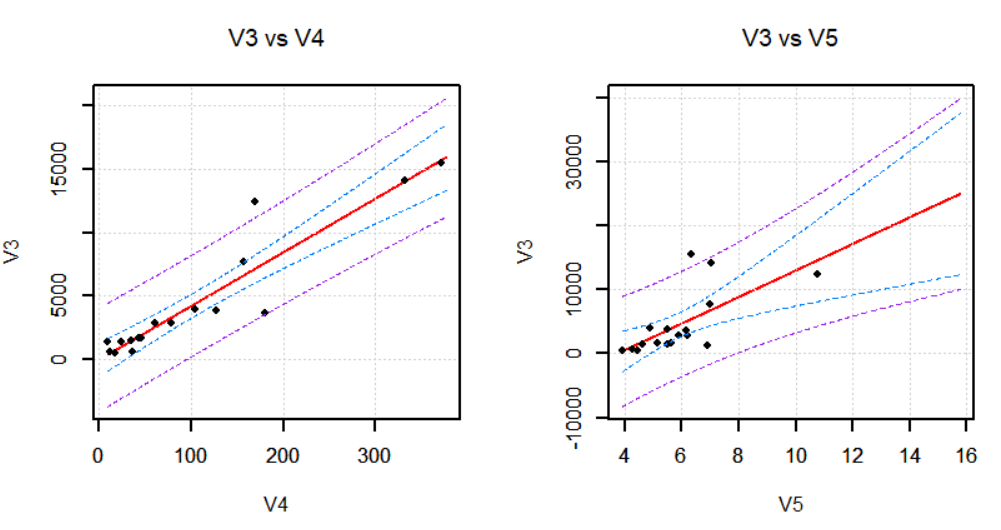
\includegraphics[scale = 0.65]{Imagen4Ej1T6.png}
 \caption{Gráficos de dispersión de las variables independientes \(\kis{V4,V5}\) contra la variable independiente \(V3\). Se deja recta de regresión lineal (recta roja) e intervalos de confianza al \(95\%\) (rectas azules) y predicción al \(95\%\) confianza (rectas purpuras).}
\label{fig:4}
\end{figure}
\begin{figure}[htb]
 \centering
 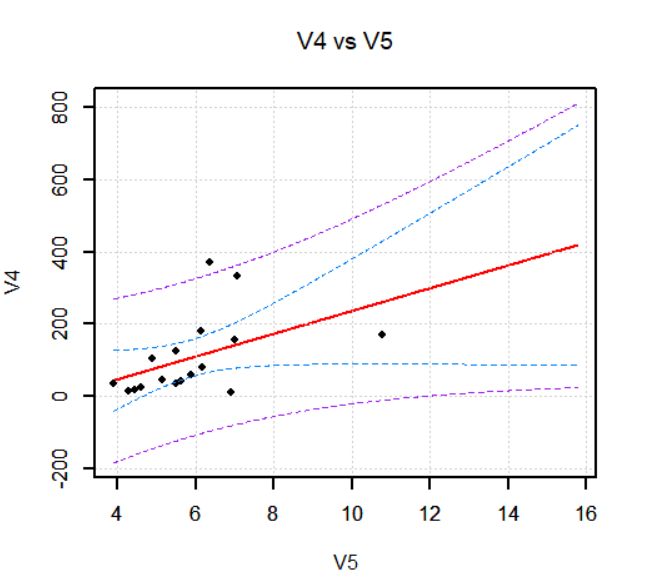
\includegraphics[scale = 0.65]{Imagen5Ej1T6.png}
 \caption{Gráfico de dispersión de la variable independiente \(V5\) contra la variable independiente \(V4\). Se deja recta de regresión lineal (recta roja) e intervalos de confianza al \(95\%\) (rectas azules) y predicción al \(95\%\) confianza (rectas purpuras).}
\label{fig:5}
\end{figure}

\noindent \textbf{b) y c)} Para \(i \in \kis{1,\hdots,5}\) se define el vector columna de datos \(X_i\) como aquel que resulta de centrar el vector columna \(Vi\) y posteriormente escalar el vector resultante dividiendo por su longitud.\footnote{Entiéndase por longitud su norma euclideana.} Sea ahora \(\mathbf{X} = \begin{pmatrix}  X_1 & X_2 & \hdots & X_5\end{pmatrix}\) se ajustará inicialmente el modelo\footnote{El centrar y escalar tiene dos propósitos en este trabajo, el evitar que los problemas generados por las diversas escalas afecten los diagnósticos de multicolinealidad, y el poder hacer comparables los modelos calculados en los ejercicios 1 y 2, con aquellos que se calcularan en los ejercicios 3 y 4, en los cuales será preferible el escalar \(\mathbf{X}\) de modo que \(\mathbf{X}'\mathbf{X}\) resulte una matriz de correlación.} 
\begin{equation}\label{1.0}
    E[W_{i}| X_{i1}, \hdots, X_{i5}] = \alpha + \delta_{1} X_{1i} + \hdots + \delta_{5} X_{i5}, \ i \in \kis{1, \hdots, 17}.
\end{equation}
esto con la finalidad de estudiar la existencia de multicolinealidad entre todas las variables independientes.\footnote{Note que las \(X_i\) son transformaciones afines de las \(Vi\), por lo que de existir multicolinealidad entre las \(Vi\) esta se vera reflejada en las \(X_i\) y viceversa.} Bajo el modelo \eqref{1.0} se tiene que la estimación\footnote{Por mínimos cuadrados ordinarios.} para \(\alpha\) es \(\hat{\alpha} = \overline{W} = 4977.892\), por lo cual, es posible olvidarnos del intercepto y ajustar de manera equivalente el modelo
\begin{equation}\label{1.2}
    E[W_{i} - \overline{W}| X_{i1}, \hdots, X_{i5}] =  \delta_{1} X_{1i} + \hdots+ \delta_{5} X_{i5}, \ i \in \kis{1, \hdots, 17}.
\end{equation}
dicho ajuste se realizó en \(R\) mediante mínimos cuadrados para las estimaciones de los coeficientes, arrojando los resultados presentados en la tabla \ref{tab:ref1}, algunos otros detalles sobre el ajuste de este modelo también se presentan en \eqref{R^2 y AIC 1}. Observe que en este primer paso se tiene un segundo indicador\footnote{Recuerde que el primero fueron las gráficas de dispersión del inciso anterior.} de la posible existencia de multicolinealidad entre las variables independientes utilizadas para el modelo, ya que en \eqref{R^2 y AIC 1} se observa que el coeficiente de determinación del modelo ajustado \eqref{tab:ref1} es bastante alto, de hecho es casi uno, sin embargo solo el coeficiente \(\delta_2\) resulta significativamente distinto de cero bajo un nivel de significancia del \(5\%\), estos primeros indicios pese a indicarnos la existencia de multicolinealidad en el modelo no nos dicen nada sobre la gravedad de la misma, por lo que se analizarán otros indicadores importantes a continuación. Primeramente, se obtuvo la matriz de correlación de las columnas de \(\mathbf{X}\) \eqref{corr1}, en la misma es posible observar que \(X_1\) y \(X_3\) están casi perfectamente correlacionadas, lo cual ya es un indicador claro de que la colinealidad entre estas dos variables es fuerte, por otro lado, observe que hay varios coeficientes de correlación que superan al \(0.9\) los cuales corresponden en su totalidad a las correlaciones entre las variables independientes en el conjunto \(\kis{X_1,\hdots,X_4}\), de este modo, los coeficientes de correlación más pequeños son aquellos que involucran a \(X_5\) lo cual era de esperarse después de lo comentado en lo gráficos de dispersión en el inciso anterior.
\begin{table}[H]
        \centering
        \begin{tabular}{@{}l@{\hskip 0.3in}r@{\hskip 0.3in}r@{\hskip 0.3in}r@{}}
            \toprule
            Coeficiente& Estimación & \(t\)-valor& \(p\)-valor \\
            \midrule
             \(\delta_1\) &  -10175 & -0.169 &  0.8687\\  
             \(\delta_2\)&    4762 &  2.748 &   0.0177*\\ 
             \(\delta_3\) &   31159 &  0.536 &  0.6018\\  
             \(\delta_4\) &   -1818 & -0.613 &  0.5516\\  
             \(\delta_5\) &   -2495 & -1.961 &  0.0735\\
            \bottomrule
        \end{tabular}
        \caption{Resultados análisis de regresión: \(W - \overline{W}\) variable respuesta \(X_1, \hdots, X_5\) variables independientes.}
        \label{tab:ref1}
\end{table}
\begin{equation}\label{R^2 y AIC 1}
    R^2 = 0.9908, \quad AIC = 272.660. 
\end{equation}

\begin{equation}\label{corr1}
R_{\mathbbf{X}} = \bordermatrix{
   & X_1   & X_2  &  X_3   & X_4&X_5\cr
X_1& 1.000& 0.907& 0.999& 0.936 &0.671\cr
X_2& 0.907& 1.000& 0.907& 0.910 &0.447\cr
X_3& 0.999& 0.907& 1.000& 0.933 &0.671\cr
X_4& 0.936& 0.910& 0.933& 1.000 &0.463\cr
X_5& 0.671& 0.447& 0.671& 0.463 &1.000
  }
\end{equation}
Por otra parte, se presenta en la figura \ref{fig:6} un mapa de calor de la matriz de correlaciones \eqref{corr1} con un dendograma generado de manera automática por el comando \(heatmap\) de \(R\), utilizando un algoritmo de machine learning conocido como hierarchical clustering, los clusters formados se basan en que tan cercanas son las distintas variables independientes utilizando como distancia a la correlación existente entre las mismas, mediante este agrupamiento es posible constatar que las variables \(X_1\) y \(X_3\) están fuertemente correlacionadas, y qué posiblemente haya una colinealidad de moderada a fuerte entre estas variables independientes y las variables independientes \(X_2\) y \(X_4\).
\begin{figure}[htb]
 \centering
 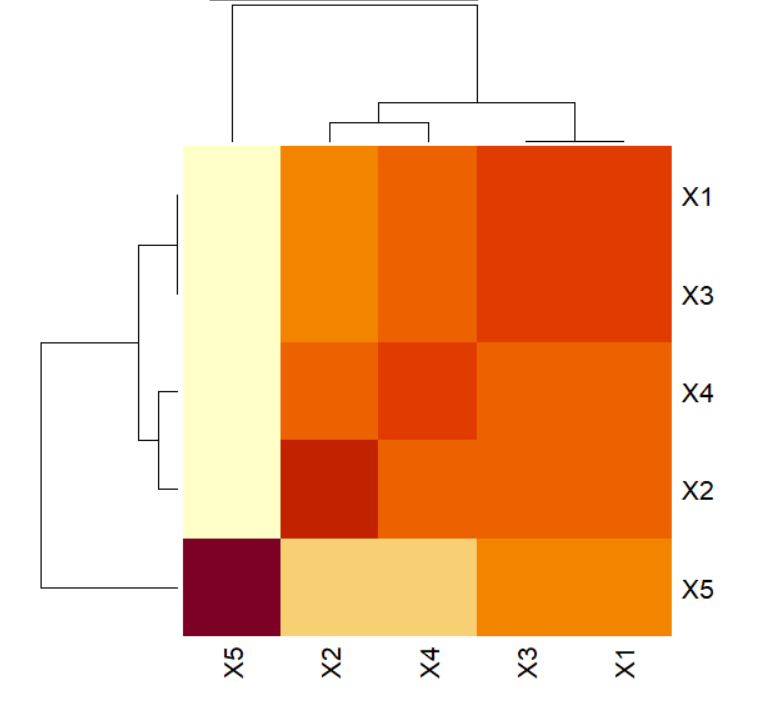
\includegraphics[scale = 0.65]{Imagen6Ej1T6.png}
 \caption{Mapa de calor de matriz de correlaciones de las columnas de \(\mathbf{X}\).}
\label{fig:6}
\end{figure}
Por otro lado, en la tabla \ref{tab:ref2} se pueden observar los factores de inflación de la varianza correspondientes a cada una de los coeficientes de nuestro modelo, note que en este caso dichos factores de inflación resultan particularmente preocupantes debido a que al menos \(3\) de ellos, los correspondientes a los coeficientes que multiplican a las variables independientes \(X_1\), \(X_3\) y \(X_4\), superan con claridad al numero \(10\) y el asociado al coeficiente que multiplica a la variable independiente \(X_2\) es mayor a \(5\), lo cual indica que estos coeficientes están siendo pobremente estimados debido a la multicolinealidad 
\begin{table}[H]
        \centering
        \begin{tabular}{@{}l@{\hskip 0.3in}r@{\hskip 0.3in}r@{\hskip 0.3in}r@{\hskip 0.3in}r@{}}
            \toprule
            \(VIF_1\)& \(VIF_2\) & \(VIF_3\)& \(VIF_4\)& \(VIF_5\) \\
            \midrule
             9598.007& 7.941 &8933.566  & 23.293&    4.280\\  
            \bottomrule
        \end{tabular}
        \caption{Factores de inflación de la varianza, modelo \ref{tab:ref1}.}
        \label{tab:ref2}
\end{table}
De igual modo, se realizó un análisis utilizando los valores propios de la matriz \(\mathbf{X}'\mathbf{X}\) con los cuales se obtuvo el número de condición de la matriz \(\mathbf{X}'\mathbf{X}\) de la siguiente manera, sea \(\lambda_{\max}\) el máximo valor propio de la matriz \(\mathbf{X}'\mathbf{X}\) y \(\lambda_{\min}\) el mínimo de ellos entonces el número de condición de la matriz \(\mathbf{X}'\mathbf{X}\) esta dado por:
\begin{equation}\label{condNum 1}
    K(\mathbf{X}'\mathbf{X}) = \frac{\lambda_{\max}}{\lambda_{\min}} =  77773.50.
\end{equation}
Dado que este número es mayor a \(1000\) se considera que existe multicolinealidad severa en las columnas de la matriz de diseño. Por último, se llevó a cabo de acuerdo a Belsey y Kuh un procedimiento conocido como descomposición de varianza, en el cual se descompone la varianza de los estimadores\footnote{Entiéndase la parte constante que multiplica al valor desconocido de \(\sigma^2\).} de los coeficientes del modelo de acuerdo a los valores singulares de la matriz \(\mathbf{X}\), que son simplemente las raíces cuadradadas positivas de lo valores propios de la matriz \(\mathbf{X}'\mathbf{X}\), este procedimiento está fuertemente relacionado con los índices de condición (ó condicionamiento) de la matriz \(\mathbf{X}'\mathbf{X}\), los cuales se obtienen de la siguiente manera, sean \(\kis{\lambda_1, \hdots, \lambda_5}\) los valores propios ordenados de manera ascendente de la matriz \(\mathbf{X}'\mathbf{X}\), entonces \(\kis{\lambda_{1}^{1/2}, \hdots, \lambda_{5}^{1/2}}\) es el conjunto de valores singulares de la matriz \(\mathbf{X}\), y los índices de condición de la matriz \(\mathbf{X}'\mathbf{X}\) se calculan como \(i_{j}=
\lambda_{5}/\lambda_{j}, \ j = 1,\hdots,5\), observe que a cada valor singular le corresponde un índice de condición, así que para hacer referencia de la proporción de varianza asociada a un valor singular de la matriz \(\mathbf{X}\) se hará referencia al porcentaje de varianza asociado a su índice de condición. Los índices de condición junto con la descomposición de varianzas mencionada y los valores singulares de \(\mathbf{X}\) correspondientes a cada índice se encuentran expuestos en la tabla \ref{tab:ref3} 
\begin{table}[H]
        \centering
\scalebox{0.8}{
\begin{tabular}{@{}l@{\hskip 0.3in}r@{\hskip 0.3in}r@{\hskip 0.3in}r@{\hskip 0.3in}r@{\hskip 0.3in}r@{\hskip 0.3in}r@{}}
\toprule
Valor Singular& \(V(\hat{\delta}_1)\)  & \(V(\hat{\delta}_2)\)  & \(V(\hat{\delta}_3)\) & \(V(\hat{\delta}_4)\) & \(V(\hat{\delta}_5)\)&  Índice de Cond.\\
\midrule
2.05  &  \(5.85\cdot10^{-6}\) &\(6.16\cdot 10^{-3}\)& \(6.27\cdot 10^{- 6}\)& \(2.17\cdot 10^{-3}\)& \(6.20\cdot 10^{-3}\)  &           1.00\\  
0.817 &  \(6.42\cdot10^{-10}\) &0.0213 & \(1.22\cdot 10^{- 10}\) & \(6.21\cdot 10^{-3}\)& 0.277 &              2.51\\
0.308 &  \(3.04\cdot10^{-5}\) &0.861 &  \(2.80\cdot 10^{- 5}\) & 0.131   &0.0328    &          6.66\\
0.202  & \(5.61\cdot10^{-4}\) &0.109  &\(7.13\cdot 10^{- 4}\) & 0.424   &0.485       &       10.15\\
\(7.35\cdot10^{-3}\) &\(9.99\cdot 10^{- 1}\)& \(3.13\cdot 10^{-3}\)& \(9.99\cdot10^{-1}\) &0.437 &  0.199&             278.88\\
            \bottomrule
        \end{tabular}}
\caption{Matriz de descomposición de varianzas.}
\label{tab:ref3}
\end{table}
La forma de obtener las proporciones de varianza asociadas a cada valor singular es un procedimiento complejo que se puede consultar en el libro de Belsey y Kuh\footnote{Referencia 3, pp. 100 - 107.}. Una vez teniendo la tabla anterior, el procedimiento se basa en ver cuales índices de condición exceden\footnote{Este criterio es coherente en el sentido de que el máximo índice de condición es igual a la raíz cuadrada del número de condición, y si el número de condición excede a \(1000\) entonces el máximo índice de condición excede a \(30\).} el \(30\), y fijarse en cuales coeficientes concentran los mayores porcentajes de varianza en estos índices, lo que es un indicativo de que las variables asociadas a dichos coeficientes presentan problemas de multicolinealidad. En este caso observe que únicamente el último índice de condicionamiento excede el \(30\), y se tiene que tanto el coeficiente de \(X_1\) como el coeficiente de \(X_3\) concentran casi el \(100\%\) de su variabilidad en dicho índice, lo que no es de sorprender y coincide con lo ya comentado hasta este punto, se destaca además que el coeficiente de \(X_4\) pareciera tener una buena proporción de variabilidad asignada a este índice de condición\footnote{Al hacer referencia a un buen porcentaje de su variabilidad, se entenderá la regla de dedo siguiente \(0.4\) o más.}. Las conclusiones de todo este análisis se presentan en el siguiente inciso. \\ 

\noindent \textbf{d)} Después de todo el análisis realizado en el inciso anterior, es claro que solo es posible quedarnos con la variable independiente \(X_1\) o con la variable independiente \(X_3\) debido a alta colinealidad que tienen, por lo que, parece ser una buena idea considerar un modelo reducido primeramente eliminando a una de estas variables, analizando detenidamente el mapa de calor de la matriz de correlación de las columnas de \(\mathbf{X}\) y los factores de inflación de la varianza presentados en la tabla \ref{tab:ref3}, se considera que la mejor opción es deshacernos de la variable \(X_1\) por tener el mayor \(VIF\) y por presentar además problemas de multicolinealidad con las demás variables independientes, por otro lado, dado que la variable independiente \(X_4\) apareció en el análisis de descomposición de la varianza como otra variable independiente que podría tener problemas de multicolinealidad con \(X_3\), aunado al hecho de que la correlación entre \(X_3\) y \(X_4\) es igual a \(0.933\) y observando que la correlación entre \(X_3\) y \(X_2\) es de \(0.907\) y la de \(X_2\) con \(X_4\) es de \(0.910\); se piensa que estas variables pueden representar problemas de multicolinealidad\footnote{Estas relaciones inclusive se ven marcadas en el mapa de calor de la matriz de correlaciones de las columnas de \(\mathbf{X}\).} de incluirse mas de una ellas en el modelo, por lo que, se decidió construir un modelo que únicamente considerará a alguna de ellas y a \(X_5\) que es la única variable independiente que no pareciera tener problemas de multicolinealidad fuerte con ninguna de las demás variables independientes, en la tabla \ref{tab:improvisada} se puede ver el coeficiente de determinación \(R^2\) y el \(AIC\) de cada uno de estos modelos de regresión lineal ajustados por mínimos cuadrados 
\begin{table}[H]
        \centering
        \begin{tabular}{@{}l@{\hskip 0.3in}r@{\hskip 0.3in}r@{\hskip 0.3in}r@{}}
            \toprule
            Variables consideradas& \(X_2\) y \(X_5\) & \(X_3\) y \(X_5\)& \(X_4\) y \(X_5\) \\
            \midrule
            \(R^2\) &0.9239  & 0.9847 &0.9104 \\  
            \(AIC\) &302.619  &275.302 &305.394 \\  
            \bottomrule
        \end{tabular}
        \caption{Coeficientes de determinación y AIC de los ajustes por mínimos cuadrados para los modelos propuestos.}
        \label{tab:improvisada}
\end{table}
Dado que el modelo que considera únicamente a las variables independientes \(X_3\) y \(X_5\) es claramente superior a los otros dos modelos en todos los aspectos considerados en la tabla \ref{tab:improvisada} se decidió presentar este en el siguiente inciso.\\ 

\noindent \textbf{e)} El modelo reducido a considerar es 
\begin{equation}\label{reducido1}
   E[W_{i} - \overline{W}| X_{i3}, X_{i5}] =  \delta_{1}' X_{3i} + \delta_{2}' X_{5i}, \ i \in \kis{1, \hdots, 17},
\end{equation}
para el cual se obtuvieron con el uso de \(R\) las estimaciones por mínimos cuadrados y los diagnósticos presentados en la tabla \ref{tab:ref4} y en \eqref{R^2 y AIC 2}
\begin{table}[H]
        \centering
        \begin{tabular}{@{}l@{\hskip 0.3in}r@{\hskip 0.3in}r@{\hskip 0.3in}r@{}}
            \toprule
            Coeficiente& Estimación & \(t\)-valor& \(p\)-valor \\
            \midrule
            \(\delta_{1}'\)&  24189.2   &  25.282 & \(1.03\cdot 10^{-13}\)\\
            \(\delta_{2}'\)& -3362.5   &   -3.514& \(3.13\cdot 10^{-3}\)\\ 
            \bottomrule
        \end{tabular}
        \caption{Resultados análisis de regresión: \(W - \overline{W}\) variable respuesta, \(X_3, X_5\) variables independientes.}
        \label{tab:ref4}
\end{table}
\begin{equation}\label{R^2 y AIC 2}
    R^2 = 0.9847, \quad AIC = 275.302.
\end{equation}
Observe que para este modelo, todos los coeficientes resultan significativamente distintos de cero bajo un nivel de significancia del \(5\%\), más aún, se tiene un coeficiente de determinación \(R^2\) aceptable y a pesar de que hubo un incremento en el \(AIC\) comparado con el modelo ajustado en el inciso b) \eqref{R^2 y AIC 1}, este incremento es muy pequeño considerando la gran cantidad de variables que se quito al modelo. Además, se analizaron nuevamente algunos de los distintos índices de multicolinealidad presentados en el inciso c) entre los cuales se destacan los siguientes. Sea  \(\mathbf{X}_1 = \begin{pmatrix} X_3 & X_5\end{pmatrix}\) la matriz de diseño para el nuevo modelo se tiene que la matriz de correlación de las columnas de \(\mathbf{X}_1\) esta dada por
\begin{equation}\label{corr 2}
R_{\mathbf{X}_{1}} = \bordermatrix{
   & X_3  & X_5\cr
X_3& 1.000& 0.671\cr
X_5& 0.671& 0.447
  }
\end{equation}
note que la correlación entre \(X_3\) y \(X_5\) pareciera no ser tan elevada, por lo menos no como algunas de las correlaciones presentadas en el inciso \textbf{c)} para el modelo completo. Por otro lado, el indice de condición de la matriz \(\mathbf{X}_{1}'\mathbf{X}_{1}\) esta dado por
\begin{equation}\label{condNum 2}
      K(\mathbf{X}_{1}'\mathbf{X}_{1}) =   5.081.
\end{equation}
El mismo es menor a \(100\), por lo que colinealidad que pudiera existir entre \(X_3\) y \(X_5\) no considerarse como un problema serio para el modelo. Por otra parte, dado que este número de condición coincide con el cuadrado del mayor índice de condicionamiento, se concluye que no será necesario realizar un procedimiento de descomposición de la varianza, debido a que la raíz cuadrada de \eqref{condNum 2} es igual a \(2.254\) y esta cantidad es claramente menor a \(30\), lo que implica que ningún índice de condicionamiento podrá ser mayor a 30. Por último, los factores de inflación de la varianza se presentan en el cuadro \ref{tab:ref5} en los mismos se observa que ninguno excede el \(5\), por lo cual no pareciera que la colinealidad entre \(X_3\) y \(X_5\), sea un problema para las estimaciones producidas por este modelo. 
\begin{table}[H]
        \centering
        \begin{tabular}{@{}l@{\hskip 0.3in}r@{\hskip 0.3in}r@{}}
            \toprule
            \(VIF_3\)& \(VIF_5\) \\
            \midrule
             1.819 &1.819 \\  
            \bottomrule
        \end{tabular}
        \caption{Factores de inflación de la varianza, modelo \ref{tab:ref1}.}
        \label{tab:ref5}
\end{table}

\noindent \textbf{Adicional} Si gusta regresar de este modelo a uno que considere las escalas originales para las variables independientes, la variable respuesta sin centrar y que se base en el que ya fue construido, basta tomar los coeficientes estimados \(2583.212\) para el intercepto \(1.232\) para el coeficiente que multiplica a la variable independiente \(V3\) y \(-530.676\) para la  el coeficiente restante.  
\end{solucion}
%%%%%%%%%%%%%%%%%%%%%%%%%%%%%%%%%%%%%%%%%%%%%%%%%%%%%%%%%%%
\begin{exo}[Datos de Evolución Calorífica del Cemento]
Los datos de la tabla \ref{tab:2}
están relacionados con la evolución calorífica en calorías por gramo de cemento
(\(y\)), como una función de las cantidades de cada uno de los siguientes cuatro
ingredientes que participan en la mezcla. Aluminato tricálcico (\(x_1\)), silicato
tricálcilo (\(x_2\)), ferrita de alumino tetracálcico (\(x_3\)), silicato dicálcico (\(x_4\)). Hacer lo siguiente
\begin{itemize}
    \item[a)] Obtenga la matriz de las correlaciones entre los regresores \(x_1\), \(x_2\), \(x_3\) y \(x_4\).
    \item[b)] Calcule los factores de inflación de la varianza.
    \item[c)] Calcule los eigenvalores de la matriz \(X'X\) también calcule el número de
condición \(K\). Interprete los valores propios de la matriz \(X'X\).
    \item[d)]De acuerdo a los resultados obtenidos en los incisos anteriores ¿sospecha
usted que la multicolinealidad está presente en los datos? ¿Qué puede decir
de la fuente de la multicolinealidad?
    \item[e)] Discuta la posibilidad de obtener modelos de regresión donde el impacto de la multicolinealidad sea menor que en el modelo completo original con las cuatro variables regresoras.
    \item[f)]Proponga un modelo de regresión en el que la multicolinealidad es menor
que en el modelo original.
\end{itemize}
\end{exo}
 \begin{table}[htbp]
        \caption{Datos de Evolución Calorífica del Cemento.}
        \centering\begin{tabular}{@{}l@{\hskip 0.3in}r@{\hskip 0.3in}r@{\hskip 0.3in}r@{\hskip 0.3in}r@{\hskip 0.3in}r@{}}
            \toprule
            $obs$ & $x_1$ & $x_2$ & $x_3$ &\(x_4\) &\(y\)\\
            \midrule
  1  &   7   &  26  &    6   &  60  &  78.5\\
  2  &     1 &    29 &    15 &    52 &   74.3\\
  3    &  11 &    56 &     8 &    20 &  104.3\\
  4     & 11 &    31 &     8 &    47 &   87.6\\
  5   &    7  &   52 &     6 &    33 &   95.9\\
  6    &  11  &   55  &    9 &    22 &  109.2\\
  7     &  3  &   71  &   17 &     6 &  102.7\\
  8   &    1  &   31  &   22 &    44 &   72.5\\
  9    &   2  &   54  &   18 &    22 &   93.1\\
 10     & 21  &   47  &    4 &    26 &  115.9\\
 11  &     1  &   40  &   23&     34 &   83.8\\
 12   &   11  &     66&      9 &  12&   113.3\\
 13     & 10  &     68&      8&   12&   109.4\\
            \bottomrule
        \end{tabular}
        \label{tab:2}
\end{table}
\begin{solucion}
\noindent \textbf{a)} El objetivo a lo largo de este ejercicio será determinar un modelo de regresión lineal para la respuesta \(y\), utilizando las variables independientes \(x_1\), \(x_2\), \(x_3\) y \(x_4\) de alguna manera, pero primero se deberá determinar si existen problemas severos de multicolinealidad entre las variables independientes los cuales puedan afectar las estimaciones del modelo. Con esto en mente, en la figura \ref{fig:7} se pueden ver todos los elementos que se encuentran por encima de la diagonal de la matriz de correlación de \(x_1\), \(x_2\), \(x_3\) y \(x_4\), debido que los elementos de la diagonal de la misma son iguales a uno y dada la simetría de la matriz de correlación, esto es suficiente para determinar la matriz de correlación completa, observe que las correlaciones más altas se encuentran señaladas con un asterisco, dichas correlaciones son la correspondiente a \(x_1\) y \(x_3\) con un valor de \(-0.824\) y la correspondiente a \(x_2\) y \(x_4\) con un valor de \(-0.973\), note que esto se ve reflejado en las correspondientes gráficas de dispersión, sobre todo en los modelos de regresión lineal ajustados para estos datos, ya que los modelos asociados a las variables independientes mencionadas son los que parecen tener los intervalos de confianza con la menor variabilidad entre todas los modelos de regresión lineal presentados.\\      
\begin{figure}[htb]
 \centering
 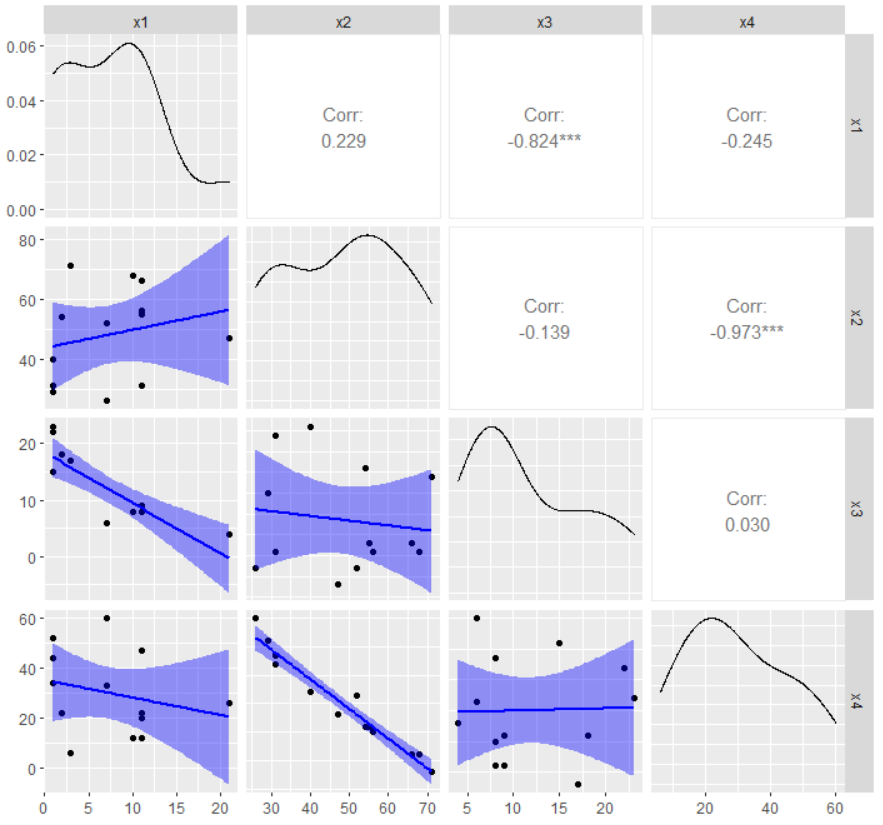
\includegraphics[scale = 0.65]{Im1Ej2T6.png}
 \caption{PairPlot con correlaciones de las variables independientes \(x_1,x_2,x_3\) y \(x_4\).}
\label{fig:7}
\end{figure}

\noindent \textbf{b)} Para \(i \in \kis{1,\hdots,4}\) se define el vector columna de datos \(X_i\) como aquel que resulta de centrar el vector columna \(x_i\) y posteriormente escalar el vector resultante dividiendo por su longitud. Sea ahora \(\mathbf{X} = \begin{pmatrix}  X_1 & X_2 & X_3 & X_4\end{pmatrix}\) se ajustará inicialmente el modelo\footnote{Ya se explicó el porque de centrar y escalar.} 
\begin{equation}\label{2.0}
    E[y_{i}| X_{i1}, \hdots X_{i4}] = \alpha + \alpha_{1} X_{1i} + \hdots \alpha_{4} X_{i4}, \ i \in \kis{1, \hdots, 13}.
\end{equation}
esto con la finalidad de estudiar la existencia de multicolinealidad entre todas las variables independientes. Bajo el modelo \eqref{2.0} se tiene que la estimación\footnote{Por mínimos cuadrados ordinarios.} para \(\alpha\) es \(\hat{\alpha} = \overline{y} = 95.423\), por lo cual, es posible olvidarnos del intercepto y ajustar de manera equivalente el modelo
\begin{equation}\label{2.2}
    E[y_{i} - \overline{y}| X_{i1}, \hdots X_{i4}] =  \alpha_{1} X_{1i} + \hdots+ \alpha_{4} X_{i4}, \ i \in \kis{1, \hdots, 13}.
\end{equation}
dicho ajuste se realizó en \(R\) utilizando estimación por mínimos cuadrados para los coeficientes del mismo arrojando los resultados presentados en la tabla \ref{tab:ref10} y en \eqref{R^2 y AIC 3}
\begin{table}[H]
        \centering
        \begin{tabular}{@{}l@{\hskip 0.3in}r@{\hskip 0.3in}r@{\hskip 0.3in}r@{}}
            \toprule
            Coeficiente& Estimación & \(t\)-valor& \(p\)-valor \\
            \midrule
\(\alpha_1\) &   31.607 &    2.209&   0.0545 \\
\(\alpha_2\) & 27.500   &    0.748&    0.4738 \\ 
\(\alpha_3\)  &  2.261  &   0.143 &  0.8893 \\
\(\alpha_4\)  & -8.353  &   -0.215 &  0.8342\\ 
            \bottomrule
        \end{tabular}
        \caption{Resultados análisis de regresión: \(y - \overline{y}\) variable respuesta \(X_1, \hdots, X_4\) variables independientes.}
        \label{tab:ref10}
\end{table}
\begin{equation}\label{R^2 y AIC 3}
    R^2 = 0.9824, \quad AIC = 63.837.
\end{equation}
Aquí podemos encontrar un segundo indicio de la existencia de multicolinealidad entre las variables independientes, esto porque ninguno de los coeficientes resulta ser significativamente distinto de cero bajo un nivel de significancia del \(5\%\), sin embargo, el coeficiente de determinación \(R^2\) del modelo resulta bastante elevado. Por otro lado, se calcularan los factores de inflación de la varianza asociados a los coeficientes del modelo, calculando primeramente la matriz de correlación de las columnas de \(\mathbf{X}\) la cual coincide con la matriz de correlación expuesta en el inciso \textbf{a)}, con el objetivo de no repetir información se presenta únicamente un mapa de calor de la misma, con un dendográma construido utilizando hierarchical clustering con el que se pueden apreciar las relaciones anteriormente\footnote{Anteriormente en su versión no escalada ni centrada.} expuestas entre las variables independientes \(X_1\) y \(X_3\) y las variables independientes \(X_2\) y \(X_4\). Posteriormente, se utilizó la diagonal de la inversa de esta matriz de correlación con lo cual se obtuvieron los factores de inflación de la varianza mencionados, los cuales se presentan en la tabla \ref{tab:ref11}, estos factores son un signo de alerta debido a que ninguno es menor en magnitud al número \(10\), por lo que se concluye que todos los coeficientes del modelo están siendo pobremente estimados debido a la multicolinealidad existente entre las variables independientes. 
\begin{figure}[htb]
 \centering
 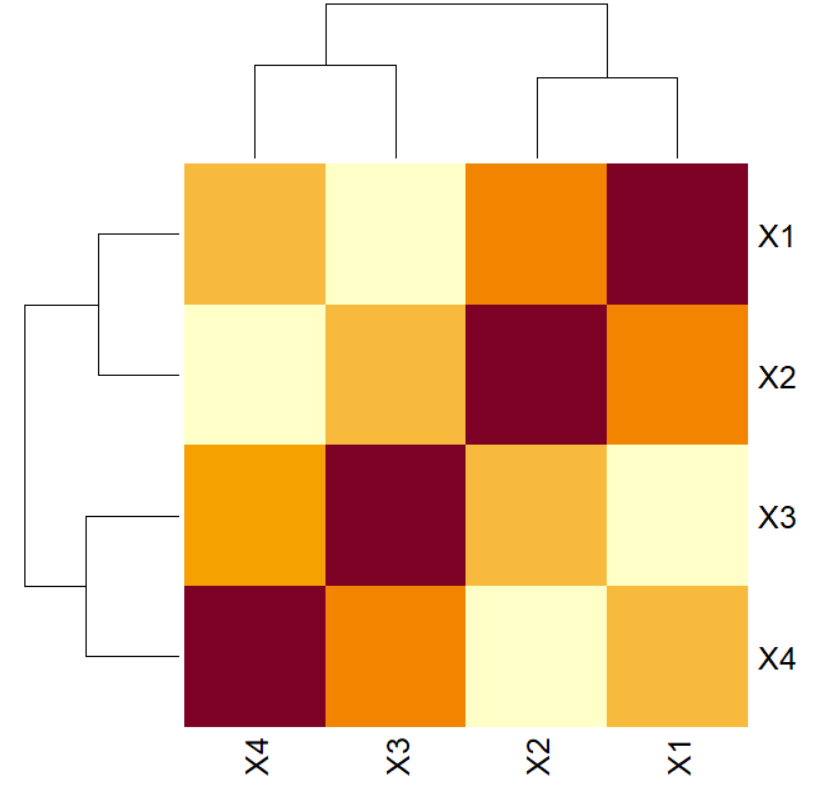
\includegraphics[scale = 0.65]{Im2Ej2T6.png}
 \caption{Mapa de calor de la matriz de correlaciones de las columnas de \(\mathbf{X}\).}
\label{fig:8}
\end{figure}
\begin{table}[H]
        \centering
        \begin{tabular}{@{}l@{\hskip 0.3in}r@{\hskip 0.3in}r@{\hskip 0.3in}r@{}}
            \toprule
            \(VIF_1\)& \(VIF_2\) & \(VIF_3\)& \(VIF_4\) \\
            \midrule
            38.496 &254.423  &46.868 &282.513 \\  
            \bottomrule
        \end{tabular}
        \caption{Factores de inflación de la varianza, modelo \ref{tab:ref1}.}
        \label{tab:ref11}
\end{table}
\noindent \textbf{c)} Los valores propios de la matriz \(\mathbf{X}'\mathbf{X}\) ordenados en forma ascendente se encuentran dados en la tabla \ref{tab:ref11}
\begin{table}[H]
        \centering
        \begin{tabular}{@{}l@{\hskip 0.3in}r@{\hskip 0.3in}r@{\hskip 0.3in}r@{}}
            \toprule
            \(\lambda_1\)& \(\lambda_2\) & \(\lambda_3\)& \(\lambda_4\) \\
            \midrule
           \(1.623\cdot10^{-3}\) &0.187& 1.576& 2.236 \\  
            \bottomrule
        \end{tabular}
        \caption{Factores de inflación de la varianza, modelo \ref{tab:ref1}.}
        \label{tab:ref11}
\end{table}
Por si solos estos valores propios no son muy interpretables, pero serán de utilidad para realizar cálculos similares a los hechos anteriormente en el inciso \textbf{c)} del ejercicio 1, para determinar la gravedad de la multicolinealidad entre las variables independientes. En primera instancia observe que el número de condición de la matriz \(\mathbf{X}'\mathbf{X}\) esta dado por
\begin{equation}\label{numCond 3}
    K(\mathbf{X}'\mathbf{X}) = \frac{\lambda_4}{\lambda_1}= 1376.881. 
\end{equation}
Debido a que el número de condición de la matriz \(\mathbf{X}'\mathbf{X}\) es mayor a \(1000\) se puede decir que la multicolinealidad existente entre las variables independientes del modelo es severa. Por lo cual, se decidió utilizar el procedimiento de descomposición de la varianza, el cual ya fue previamente explicado en el ejercicio anterior, los resultados de este procedimiento están expuestos en la tabla \ref{tab:ref12}
\begin{table}[H]
        \centering
\scalebox{0.9}{
\begin{tabular}{@{}l@{\hskip 0.3in}r@{\hskip 0.3in}r@{\hskip 0.3in}r@{\hskip 0.3in}r@{\hskip 0.3in}r@{}}
Valores Singulares& \(V(\hat{\alpha}_1)\)&  \(V(\hat{\alpha}_2)\)& \(V(\hat{\alpha}_3)\)& \(V(\hat{\alpha}_4)\) & Índice de Cond\\
\toprule
1.50  & \(2.63\cdot10^{-3}\)& \(5.59\cdot10^{-4}\) &\(1.48\cdot10^{-3}\) &\(4.75\cdot10^{-4}\)  &1.000  \\ 
1.26  & \(4.27\cdot10^{-3}\)& \(4.27\cdot10^{-4}\) &\(4.95\cdot10^{-3}\) &\(4.57\cdot10^{-4}\)  &1.191 \\
0.432 & 0.0635 & \(2.08\cdot10^{-3}\)  &0.0465  &\(7.24\cdot10^{-4}\)  &3.461\\
0.0403& 0.930  & 0.997&0.947 &0.998     &37.106 \\
            \bottomrule
        \end{tabular}}
\caption{Matriz de descomposición de varianzas.}
\label{tab:ref12}
\end{table}
En la tabla \ref{tab:ref12} podemos observar que el único índice de condicionamiento que supera al \(30\) es el último, el cual coincide con la raíz cuadrada positiva del número de condición de la matriz \(\mathbf{X}'\mathbf{X}\), y que todos los estimadores de los coeficientes tienen casi el \(100\%\) de su varianza concentrada en este índice, por lo que todas las variables independientes parecen padecer de problemas por la multicolinealidad. Las conclusiones de los análisis hechos hasta el momento se presentan en el siguiente inciso. \\ 

\noindent \textbf{d)} Se observó que todas las variables independientes presentan en este modelo problemas de multicolinealidad los cuales afectan por ejemplo a las estimaciones de los coeficientes del modelo, como ya se mencionó cuando se realizaron los cálculos de los \(VIF\), sin embargo, se notó en repetidas ocasiones que la multicolinealidad en el modelo parece ser una consecuencia de la relación existente entre las variables independientes \(X_1\) y \(X_3\), y las variables independientes \(X_2\) y \(X_4\), de lo que se concluye que lo mas sensato sería tomar una y solo una variable entre \(X_1\) y \(X_3\) para el modelo y lo mismo para las variables \(X_2\) y \(X_4\).\\

\noindent \textbf{e)} Para este inciso se ajustaron dos modelos, el que únicamente considera como regresoras a las variables independientes \(X_1\) y \(X_2\) y el que considera como regresoras únicamente a las variables independientes \(X_3\) y \(X_4\), se destaca que el primer modelo mencionado obtuvo un coeficiente de determinación \(R^2\) igual a \(0.979\) y un \(AIC\) de \(62.312\), mientras que el segundo modelo obtuvo un coeficiente de determinación \(R^2\) de \(0.935\) y un \(AIC\) de \(76.745\), de este modo se decidió que el modelo más adecuado para este problema era el que considera como regresoras únicamente a las variables independientes \(X_1\) y \(X_2\), todos los detalles sobre este modelo se expondrán en el siguiente inciso. 

\begin{rem}
Es importante destacar que se consideraron otros modelos, con otras combinaciones de las variables regresoras de acuerdo a las conclusiones obtenidas en el inciso \textbf{d)}, sin embargo,  estos dos fueron los que obtuvieron los mejores resultados.
\end{rem}
\noindent \textbf{f)}  El modelo reducido a considerar es 
\begin{equation}\label{reducido2}
   E[y_{i} - \overline{y}| X_{i1},X_{i2}] =  \alpha_{1}' X_{1i} + \alpha_{2}' X_{2i}, \ i \in \kis{1, \hdots, 13},
\end{equation}
para el cual se obtuvieron con el uso de \(R\) las estimaciones y diagnósticos presentados en la tabla \ref{tab:ref13} y en \eqref{R^2 y AIC 4}

\begin{table}[H]
        \centering
        \begin{tabular}{@{}l@{\hskip 0.3in}r@{\hskip 0.3in}r@{\hskip 0.3in}r@{}}
            \toprule
            Coeficiente& Estimación & \(t\)-valor& \(p\)-valor \\
        \midrule
\(\alpha_{1}'\) &  29.920 &12.70& \(6.51\cdot10^{-8}\)\\
 \(\alpha_{1}'\)& 35.698 &15.15& \(1.03\cdot10^{-8}\)\\                    \bottomrule
        \end{tabular}
        \caption{Resultados análisis de regresión: \(y - \overline{y}\) variable respuesta, \(X_1, X_2\) variables independientes.}
        \label{tab:ref13}
\end{table}
\begin{equation}\label{R^2 y AIC 4}
    R^2 = 0.979, \quad AIC = 62.312.
\end{equation}
Se destaca que todos los coeficientes resultan ser significativos bajo un nivel de significancia del \(5\%\), que el coeficiente \(R^2\) es aceptable y que el \(AIC\) de este modelo mejoró un poco en comparación con el del modelo que considera a todas las variables independientes \eqref{R^2 y AIC 3}. Más aún, referente a a los temas de multicolinealidad, sea \(\mathbf{X}_{1} = \begin{pmatrix}X_1 & X_2\end{pmatrix}\) la matriz de diseño del modelo \eqref{reducido2} se tiene que la matriz de correlación de sus columnas esta dada por
\begin{equation}\label{cor 4}
R_{\mathbf{X}_{1}} = \bordermatrix{
   & X_1  & X_2\cr
X_1& 1.000 &0.229\cr
X_2& 0.229 &1.000
  }.
\end{equation}
Claramente la correlación entre \(X_1\) y \(X_2\) es considerablemente pequeña, tomando en cuenta que en valor absoluto es más cercana a cero que a uno, y además los Factores de Inflación de la varianza para los estimadores de los coeficientes de este modelo, los cuales se encuentran dados en la tabla \ref{tab:ref16}, resultan ambos menores que \(5\), por que la colinealidad entre \(X_1\) y \(X_2\) no resultará un problema en las estimaciones que se hagan de los coeficientes
\begin{table}[H]
        \centering
        \begin{tabular}{@{}l@{\hskip 0.3in}r@{\hskip 0.3in}r@{}}
            \toprule
            \(VIF_1\)& \(VIF_2\) \\
            \midrule
             1.055 &1.055  \\  
            \bottomrule
        \end{tabular}
        \caption{Factores de inflación de la varianza, modelo \ref{tab:ref1}.}
        \label{tab:ref16}
\end{table}
Por último, el número de condición de la matriz \(\mathbf{X}_{1}'\mathbf{X}_{1}\) esta dado por
\begin{equation}
    K(\mathbf{X}_{1}'\mathbf{X}_{1}) = 1.26.
\end{equation}
Dicho número de condición es mucho menor a \(100\) lo que constata que la colinealidad existente entre las variables independientes \(X_1\) y \(X_2\) es débil.\\

\noindent \textbf{Adicional} Si gusta regresar de este modelo a uno que considere las escalas originales y se base en el que ya fue construido, basta tomar los coeficientes estimados \(52.577\) para el intercepto \(1.468\) para el coeficiente que multiplica a la variable independiente \(x1\) y \(0.662\) para la  el coeficiente restante. 
\end{solucion}

\begin{rem}
A partir de este punto \(I_{p}\) representa a una matriz identidad de dimensión \(p \times p\) con \(p \in \NN\), y \(0_p\) representa un vector columna de dimensión \(p \times 1\) con todas sus entradas iguales a cero.  
\end{rem}
%%%%%%%%%%%%%%%%%%%%%%%%%%%%%%%%%%%%%%%%%%%%%%%%%%%%%%%%%%%
\begin{exo}[Análisis de datos de servicio hospitalario (Ridge Regression)]
Hacer
el análisis de los datos de la tabla \ref{tab:1} que correspondan al servicio hospitalario,
utilizando el método de regresión Ridge. Hacer lo siguiente:
\begin{itemize}
    \item[a)] Determine el valor del parámetro de sesgo \(\mathit{k}\) siguiendo el procedimiento propuesto por Hoerl et al. (1975).
    \item[b)] Determinar el valor del parámetro de sesgo \(\mathit{k}\) utilizando el método de validación cruzada
    \item[c)] Estime para ambos valores de \(\mathit{k}\) obtenidos en los incisos (a y b) los coeficientes de regresión ridge \(\beta_{(k)}\), considerando las ecuaciones normales (tipo ridge)
    \[
    (X'X + kI_{p})\hat{\beta}_{(k)} = X'Y. 
    \]
    \item[d)] Compare y comente las soluciones del inciso anterior. 
    \item[e)] Compare y comente la mejor solución del inciso (c) con el modelo propuesto en el inciso e) del problema.
\end{itemize}
\end{exo}
\begin{solucion}
\textbf{a)}
En este ejercicio se buscará ajustar el modelo \eqref{1.0} utilizando regresión de Ridge, sin embargo, de acuerdo a Hastie y Tibsharani\footnote{Ver referencia 1, pp. 64.} considerando este modelo con las variables independientes centradas y escaladas se tiene que la estimación Ridge para el intercepto esta dada por \(\hat{\alpha} = \overline{W} = 4977.892
\), y por ende es posible considerar de manera equivalente el modelo \eqref{1.2} y obtener mediante regresión Ridge las estimaciones para los coeficientes de dicho modelo utilizando la matriz de diseño \(\mathbf{X} = (X_1, \hdots, X_5)\) como fue definida en el inciso \textbf{b)} del ejercicio 1, de este modo además se cumplirá una de las condiciones estipuladas en el artículo de Hoerl (1975), es decir que la matriz de diseño \(\mathbf{X}\) estará escalada de tal suerte que \(\mathbf{X}'\mathbf{X}\) sea una matriz de correlación. Ahora, de acuerdo al artículo de Hoerl (1975) una manera de estimar el valor del parámetro de sesgo \(\mathit{k}\) que resulte óptimo\footnote{En el sentido de que este \(\mathit{k}\) sea tal que el error cuadrático promedio que comete el estimador Ridge sea el mínimo posible.} es 
\begin{equation*}
    \mathit{k_h} = \frac{p \hat{\sigma}^2}{\hat{\delta}' \hat{\delta}},
\end{equation*}
donde \(p\) es el número de parámetros en el modelo \eqref{1.2}, es decir \(p = 5\), \(\hat{\sigma}^2\) es una estimación de la varianza de los términos de error en el modelo \eqref{1.2}, la cual fue calculada usando la suma de cuadrados de los residuales del modelo \eqref{1.2} estimado por mínimos cuadrados y arrojó un valor de \(\hat{\sigma}^2 = 378270\), y \(\hat{\delta}\) es el estimador de mínimos cuadrados para los coeficientes del modelo \eqref{1.2} el cual puede encontrarse en la tabla \ref{tab:ref1}. De este modo el valor del parámetro de sesgo obtenido por este método es 
\begin{equation}\label{Kho1}
    \mathit{k_h} = 1.709\cdot 10^{-3}. 
\end{equation}

\noindent \textbf{b)} Primeramente, para determinar un rango posible en el que buscar el valor de \(\mathit{k}\) óptimo mediante validación cruzada, se realizó un gráfico de la traza de Ridge\footnote{En dicho gráfico se comete adrede un abuso de notación, ya que se omite la notación \(\hat{\delta}\) para el estimador, con la finalidad de que los elementos en la gráfica no se vean apelmazados.} el cual se presenta en la figura \ref{fig:9}, en la misma se puede observar como el vector de parámetros Ridge estimados \(\hat{\delta}_{k}\) comienza a degenerarse a cero para valores cercanos a \(10\), por lo que se esperaría que el valor óptimo para \(\mathit{k}\) se encontrará dentro del rango de 0 a 10. Por otro lado, se estimó la cota superior para este valor de \(k\) óptimo, vista en ayudantías, utilizando las cantidades calculadas en el ejercicio anterior de la siguiente manera 
\begin{equation*}
    cota = \frac{2\hat{\sigma}^2 }{\hat{\delta}'\hat{\delta}} = 6.837\cdot 10^{-4}. 
\end{equation*}
Dado que las estimaciones utilizadas para este cálculo cuentan con una variabilidad alta,\footnote{Debido a los problemas de multicolinealidad detectados en el modelo \eqref{1.2} en el ejercicio 1.}, y de acuerdo a lo observado en la traza de Ridge, se decidió buscar el \(k\) óptimo en un rango de \(0\) a \(1\). \\
\begin{figure}[htb]
 \centering
 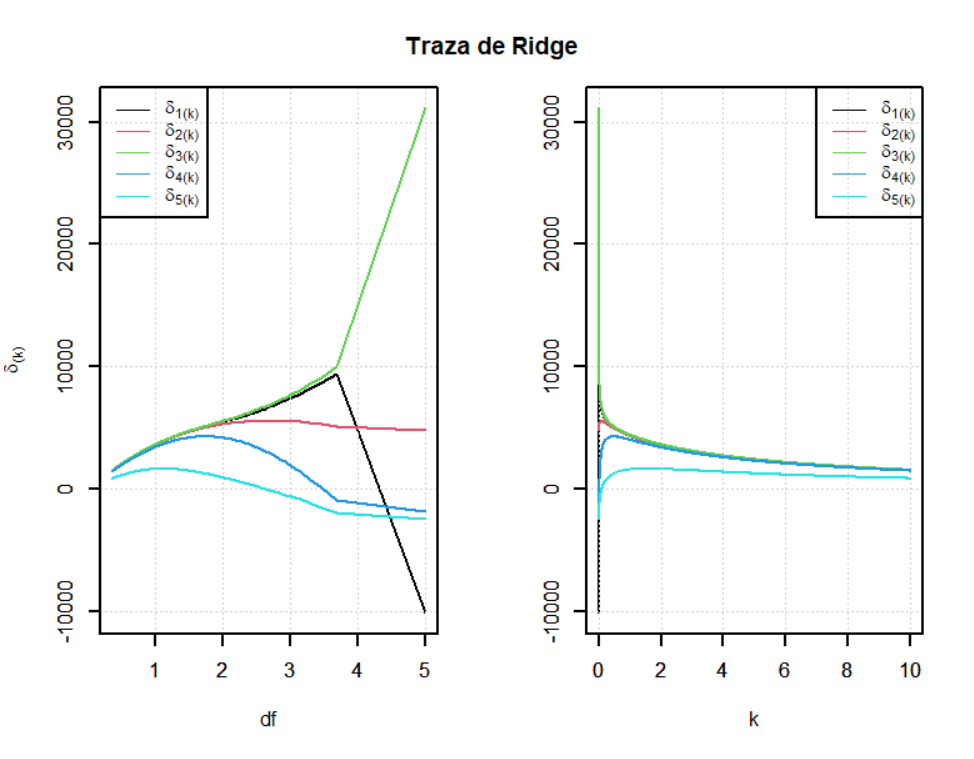
\includegraphics[scale = 0.65]{Im1Ej3T6.png}
 \caption{Gráficos de la traza de Ridge.}
\label{fig:9}
\end{figure}

Para poder llevar a cabo la validación cruzada se programó en \(R\) el método conocido como \(K\)-fold cross validation y para determinar el valor adecuado para el parámetro de sesgo \(\mathit{k}\) se utilizaron \(K = 17\) grupos realizando entonces una validación cruzada del tipo \(Leave-One-Out\), este procedimiento se repitió \(10\) veces utilizando una rejilla de \(1000\) valores entre cero y uno, dado que la estimación para el \(k\) óptimo resultaba ser menor a \(0.5\), se decidió repitir este algoritmo pero con una rejilla de \(1000\) valores entre \(0\) y \(0.5\) para intentar mejorar la precisión de la estimación, el valor resultante para \(k\) por este método fue\footnote{Este valor fue comprobado con la función \(RidgeCV\) de Python para corroborar el resultado.} 
\begin{equation}\label{k1}
    \mathit{k}_{vc} = 0.0846,
\end{equation}
Por último, se deja en la figura \ref{fig:10} una gráfica de los diversos valores de \(\mathit{k}\) entre cero y cero punto cinco utilizados y el error promedio estimado que comete el modelo en sus predicciones con dichos valores de \(\mathit{k}\).\\ 
\begin{figure}[htb]
 \centering
 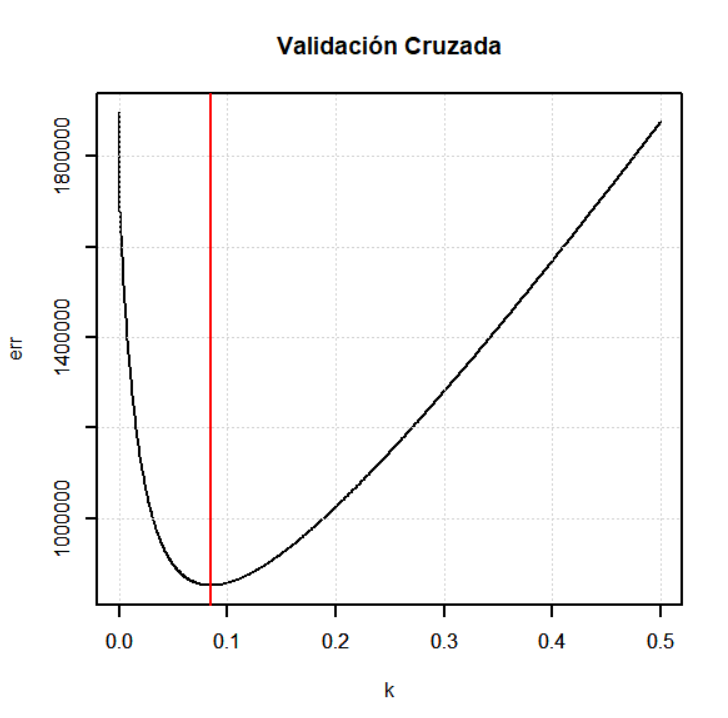
\includegraphics[scale = 0.65]{Im2Ej3T6.png}
 \caption{gráfica de los diversos valores de \(\mathit{k}\) entre cero y cero punto cinco utilizados y el error cuadrático promedio estimado que comete el modelo con dichos valores de \(\mathit{k}\). En linea roja vertical se remarca el valor óptimo para \(k\) \eqref{k1}.}
\label{fig:10}
\end{figure}

\noindent \textbf{c)} Denote por \(\hat{\delta}_{(k_{h})}\) al vector de estimaciones Ridge de los coeficientes del modelo obtenido usando el parámetro de sesgo \(k_h\), calculado en el inciso \textbf{a)} de este ejercicio, entonces se tiene que
\begin{equation*}
    \hat{\delta}_{(k_{h})} = (\mathbf{X}'\mathbf{X} + k_h I_{p})^{-1}\mathbf{X}'Y_{W} =  \begin{pmatrix}  9743.096\\
   4860.627\\
  11479.145\\
  -2156.766\\
  -2540.559\end{pmatrix},
\end{equation*}
donde \(Y_{W} = W - \overline{W} = \begin{pmatrix}W_{1} - \overline{W} & \cdots & W_{17} - \overline{W} \end{pmatrix}'\). De este modo los valores ajustados por este modelo pueden escribirse como:
\begin{equation}\label{Mod kh}
      \widehat{E}[W_{i} - \overline{W}| X_{i1}, \hdots, X_{i5}] =  9743.096 X_{1i} + \hdots-2540.559 X_{i5}, \ i \in \kis{1, \hdots, 17}.
\end{equation}

Por otra parte, denote por \(\hat{\delta}_{(k_{vc})}\) al vector de estimaciones Ridge de los coeficientes del modelo obtenido usando el parámetro de sesgo \(k_{vc}\), calculado en el inciso \textbf{b)} de este ejercicio, entonces se tiene que
\begin{equation*}
    \hat{\delta}_{(k_{vc})} = (\mathbf{X}'\mathbf{X} + k_h I_{p})^{-1}\mathbf{X}'Y_{W} =  \begin{pmatrix}  6778.872\\
 5570.405\\
 6968.747\\
 2825.609\\
-139.701\end{pmatrix}.
\end{equation*}
De este modo los valores ajustados por este modelo pueden escribirse como:
\begin{equation}\label{Mod kvc}
      \widehat{E}[W_{i} - \overline{W}| X_{i1}, \hdots, X_{i5}] =  6778.872 X_{1i} + \hdots-139.701 X_{i5}, \ i \in \kis{1, \hdots, 17}.
\end{equation}

\noindent \textbf{d)} Para este inciso se ocuparon dos criterios, el primero de ellos serán los factores de inflación de la varianza de los modelos ajustados \eqref{Mod kh} y \eqref{Mod kvc}, dichos factores de inflación de la varianza se calcularon de acuerdo a las notas del doctor Rogelio Ramos Quiroga de la siguiente manera, primero se realizaron en \(R\) los siguientes productos matriciales 
\begin{equation}\label{prod}
     (\mathbf{X}'\mathbf{X} + k I_{p})^{-1}(\mathbf{X}'\mathbf{X})(\mathbf{X}'\mathbf{X} + k I_{p})^{-1},
\end{equation}
con \(k \in \kis{k_{vc},k_{h}}\). Así, los factores de inflación de la varianza para el modelo \eqref{Mod kh} se obtuvieron como la diagonal del producto \eqref{prod} con \(k = k_{h}\) y se presentan en la tabla \ref{tab:ref20}
\begin{table}[H]
        \centering
        \begin{tabular}{@{}l@{\hskip 0.3in}r@{\hskip 0.3in}r@{\hskip 0.3in}r@{\hskip 0.3in}r@{}}
            \toprule
            \(VIF_{1}^{k_h}\)& \(VIF_{2}^{k_h}\) & \(VIF_{3}^{k_h}\)& \(VIF_{4}^{k_h}\)& \(VIF_{5}^{k_h}\) \\
            \midrule
             14.284& 7.606 &14.528 &12.236 & 3.254\\  
            \bottomrule
        \end{tabular}
        \caption{Factores de inflación de la varianza, modelo \eqref{Mod kh}.}
        \label{tab:ref20}
\end{table}
De manera análoga se obtuvieron los factores de inflación de la varianza del modelo ajustado \eqref{Mod kvc} arrojando los resultados expuestos en la tabla \ref{tab:ref21}
\begin{table}[H]
        \centering
        \begin{tabular}{@{}l@{\hskip 0.3in}r@{\hskip 0.3in}r@{\hskip 0.3in}r@{\hskip 0.3in}r@{}}
            \toprule
            \(VIF_{1}^{k_{vc}}\)& \(VIF_{2}^{k_{vc}}\) & \(VIF_{3}^{k_{vc}}\)& \(VIF_{4}^{k_{vc}}\)& \(VIF_{5}^{k_{vc}}\) \\
            \midrule
             0.708 &2.177 &0.800& 2.055& 1.217 \\  
            \bottomrule
        \end{tabular}
        \caption{Factores de inflación de la varianza, modelo ajustado \eqref{Mod kvc}.}
        \label{tab:ref21}
\end{table}
Y como segundo criterio se obtuvieron los coeficientes de determinación \(R^2\) para ambos modelos, los cuales se calcularon en Python arrojando un coeficiente de determinación 
\begin{equation}\label{R^2 1}
    R^2 = 0.9907,
\end{equation}
para el modelo ajustado \eqref{Mod kh}. Y un coeficiente de determinación 
\begin{equation}\label{R^2 2}
    R^2 = 0.9846, 
\end{equation}
para el modelo ajustado \eqref{Mod kvc}. Ahora, note que pese a que el modelo ajustado \eqref{Mod kh} posee un \(R^2\) mayor al del modelo ajustado \eqref{Mod kvc}, hay tres factores de inflación de la varianza en este modelo que superan al \(10\) y por ende, al menos tres de las estimaciones de los coeficientes estarán siendo pobremente estimados debido a problemas de multicolinealidad. Por ende, dado que uno de los principales objetivos de utilizar regresión Ridge consiste en conservar todas las variables independientes disminuyendo los problemas de multicolinealidad, se prefiere el modelo ajustado \eqref{Mod kvc} debido a que en el mismo ninguno de los factores de inflación de la varianza supera al \(10\), además de que la diferencia entre los coeficientes de determinación de ambos modelos no parece ser tan grande.\\

\noindent \textbf{e)} Observe que los factores de inflación de la varianza para el mejor modelo\footnote{Modelo ajustado \eqref{Mod kvc}.} ajustado en el inciso \textbf{c)} de este problema y los factores de inflación de la varianza del modelo \eqref{reducido1}-\eqref{tab:ref4} propuesto en el inciso \textbf{e)} del problema 1, los cuales fueron presentados en las tablas \ref{tab:ref21} y \ref{tab:ref5} respectivamente, no parecen presentar una diferencia significativa que nos haga decantarnos por uno u otro modelo, inclusive todos estos factores de inflación de la varianza resultan menores a \(5\) por lo que la multicolinealidad existente en ambos modelos no es un problema para las estimaciones de los coeficientes de los mismos. Sin embargo, observe que el coeficiente de determinación \(R^2\) del modelo ajustado \eqref{Mod kvc} es de \(0.9846\), mientras que el coeficiente de determinación del modelo propuesto en el inciso \textbf{e)}\footnote{Ver \eqref{R^2 y AIC 2}.} del ejercicio 1 es de \(0.9847\), por lo que, se concluye que el modelo propuesto en el ejercicio 1 inciso \textbf{e)} pareciera ser mejor opción, ya que utilizando un menor número de variables explicativas consigue un coeficiente de determinación superior al del mejor modelo del inciso \textbf{c)}.
\end{solucion}
%%%%%%%%%%%%%%%%%%%%%%%%%%%%%%%%%%%%%%%%%%%%%%%%%%%%%%%%%%
\begin{exo}[\shortstack{Análisis de datos de la tabla \ref{tab:2}, correspondientes a la evolución calorífica
del cemento,\\ utilizando el método de regresión Ridge}]
Hacer
el análisis de los datos de la tabla \ref{tab:2} que correspondan  a la evolución calorífica
del cemento, utilizando el método de regresión Ridge. Hacer lo siguiente:
\begin{itemize}
    \item[a)] Determine el valor del parámetro de sesgo \(\mathit{k}\) siguiendo el procedimiento propuesto por Hoerl et al. (1975).
    \item[b)] Determinar el valor del parámetro de sesgo \(\mathit{k}\) utilizando el método de validación cruzada
    \item[c)] Estime para ambos valores de \(\mathit{k}\) obtenidos en los incisos (a y b) los coeficientes de regresión ridge \(\beta_{(k)}\), considerando un procedimiento de mínimos
cuadrados ordinarios, aumentando las matrices de la siguiente forma: Sean
    \[
    X_A= \begin{pmatrix}X\\ \sqrt{\mathit{k}}I_{p}\end{pmatrix} \text{ y } Y_A = \begin{pmatrix}Y\\ 0_p\end{pmatrix},
    \]
    Las estimaciones tipo ridge de los coeficientes de regresión tipo ridge son:
    \[
    \hat{\beta}_{(k)} = (X_{A}'X_{A})^{-1}X_{A}'Y_{A}.
    \]
    \item[d)] Compare y comente las soluciones del ejercicio anterior. 
    \item[e)] Compare y comente la mejor solución del inciso (c) con el modelo propuesto en el inciso (f) del problema 2.
\end{itemize}
\end{exo}
\begin{solucion}
\textbf{a)} El objetivo de los primeros incisos de este ejercicio será estimar los coeficientes del modelo \eqref{2.0} utilizando regresión de Ridge, sin embargo, recuerde que considerando este modelo con las variables independientes centradas y escaladas se tiene que la estimación Ridge para el intercepto esta dada por \(\hat{\alpha} = \overline{y} = 95.423\), y por ende es posible considerar de manera equivalente el modelo \eqref{2.2} y obtener mediante regresión Ridge las estimaciones para los coeficientes de dicho modelo utilizando la matriz de diseño \(\mathbf{X} = (X_1, X_2, X_3, X_4)\) como fue definida en el inciso \textbf{b)} del ejercicio 2, de esto modo además se cumplirá una de las condiciones estipuladas en el artículo de Hoerl (1975), es decir que la matriz de diseño \(\mathbf{X}\) estará escalada de tal suerte que \(\mathbf{X}'\mathbf{X}\) sea una matriz de correlación. Ahora, de acuerdo al artículo de Hoerl (1975) una manera de estimar el valor del parámetro de sesgo \(\mathit{k}\) que resulte óptimo es 
\begin{equation*}
    \mathit{k_h} = \frac{p \hat{\sigma}^2}{\hat{\delta}' \hat{\delta}},
\end{equation*}
donde \(p\) es el número de parámetros en el modelo \eqref{2.2}, es decir \(p = 4\), \(\hat{\sigma}^2\) es una estimación de la varianza de los términos de error en el modelo \eqref{2.2}, la cual fue calculada usando la suma de cuadrados de los residuales del modelo \eqref{2.2} estimado por mínimos cuadrados y arrojó un valor de \(\hat{\sigma}^2 = 5.318\), y \(\hat{\alpha}\) es el vector de estimadores de mínimos cuadros el cual puede encontrarse en la tabla \ref{tab:ref10}. De este modo 
\begin{equation*}
     \mathit{k_h} = 0.0116.
\end{equation*}

\noindent\textbf{b)} Nuevamente para determinar un rango posible en el que buscar el valor de \(\mathit{k}\) óptimo mediante validación cruzada, se realizó un gráfico de la traza de Ridge\footnote{En dicho gráfico se comete adrede un abuso de notación, ya que se omite la notación \(\hat{\alpha}\) para el estimador, con la finalidad de que los elementos en la gráfica no se vean apelmazados.} el cual se presenta en la figura \ref{fig:11}, en la misma se puede observar como el vector de parámetros ridge estimados \(\hat{\alpha}_{k}\) comienza a degenerarse a cero para valores cercanos a \(35\), por lo que se esperaría que el valor óptimo para \(\mathit{k}\) se encontrará dentro del rango de \(0\) a \(35\). También se estimó la cota superior para este valor de \(k\) óptimo, aprovechando las cantidades calculadas en el ejercicio anterior de la siguiente manera 
\begin{equation*}
    cota = \frac{2\hat{\sigma}^2 }{\hat{\delta}'\hat{\delta}} = 5.812\cdot 10^{-3}.
\end{equation*}
Atendiendo a lo ocurrido en el inciso anterior, en el cual la estimación de esta cota resulto un poco pequeña para el valor del \(k\) óptimo, se decidió buscar en un rango de \(0\) a \(10\) tomando en cuenta los resultados obtenidos en la gráfica de la traza de Ridge. 
\begin{figure}[htb]
 \centering
 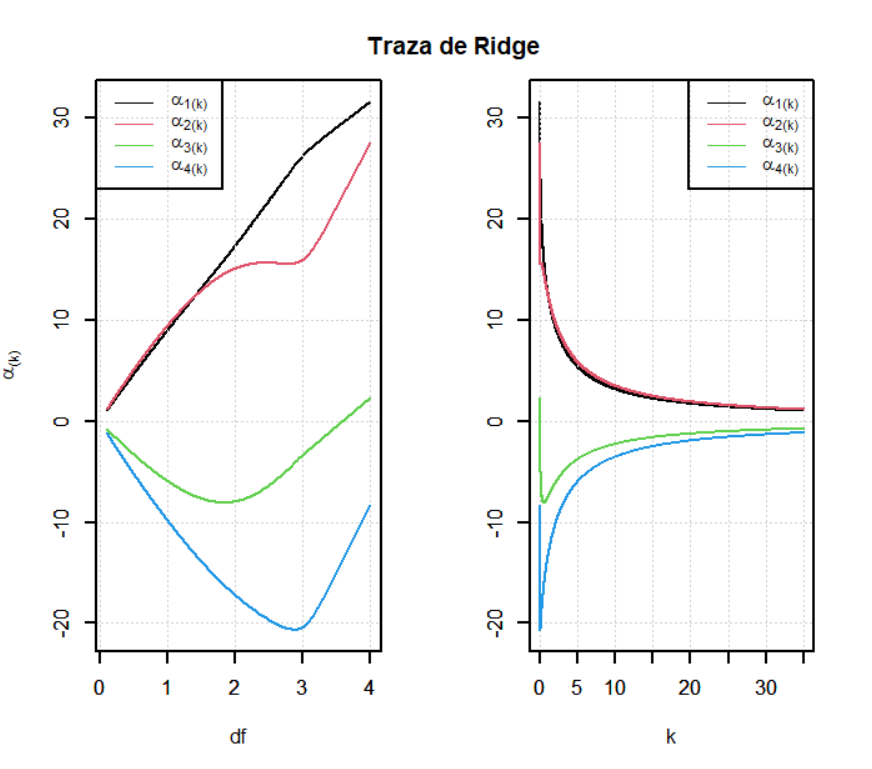
\includegraphics[scale = 0.65]{Im1Ej4T6.png}
 \caption{Gráficos de la traza de Ridge.}
\label{fig:11}
\end{figure}
De este modo, utilizando nuevamente la función programada para realizar validación cruzada, se estimó el valor de \(k\) óptimo estableciendo \(K =13\) grupos, es decir, se realizó una validación cruzada del tipo \(Leave-One-Out\) utilizando una rejilla de 1000 valores posibles para \(k\) entre \(0\) y \(10\), este se repitió 10 veces con lo que se obtuvo un valor menor a \(0.5\) para el \(k\) óptimo, de este modo se decidió volver a correr todo este algoritmo pero esta vez utilizando una rejilla de 1000 valores posibles para \(k\) entre \(0\) y \(0.5\) con la finalidad de mejorar la precisión de la estimación dada, dando como resultado el siguiente valor del parámetro de sesgo
\begin{equation*}
    k_{vc}  = 1.001\cdot 10^{-2}.
\end{equation*}
Para finalizar este inciso, puede verse en la figura \ref{fig:chtmDembelé} una gráfica de algunos de los valores de \(\mathit{k}\) entre cero y cero punto cinco utilizados y el error promedio estimado que comete el modelo en sus predicciones con dichos valores de \(\mathit{k}\).\\ 
\begin{figure}[htb]
 \centering
 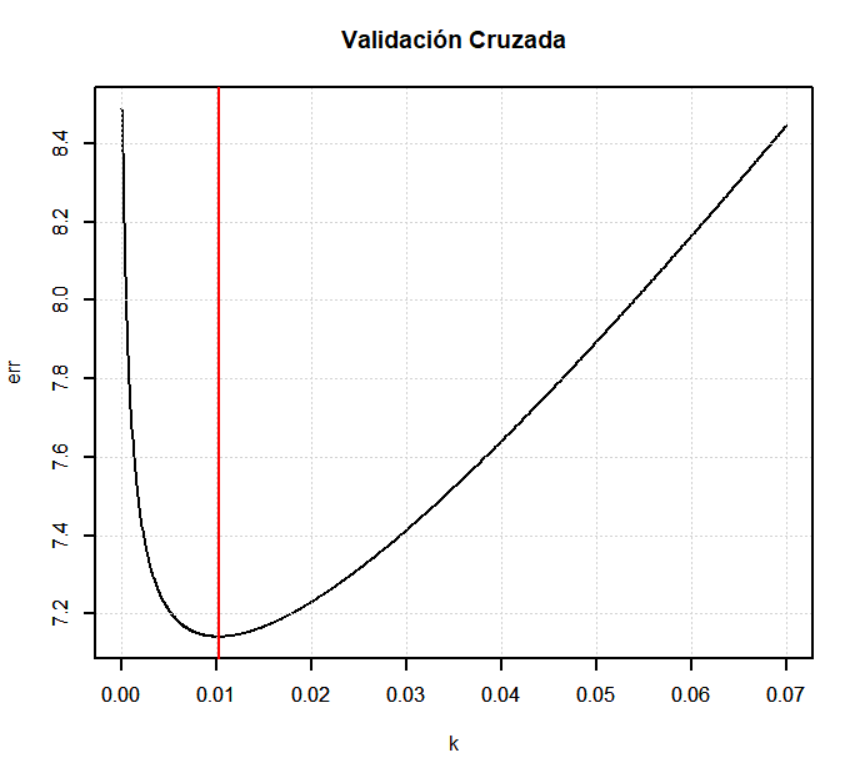
\includegraphics[scale = 0.65]{Im2Ej4T6.png}
 \caption{gráfica de los algunos valores de \(\mathit{k}\) entre cero y cero punto cinco utilizados y el error cuadrático promedio estimado que comete el modelo con dichos valores de \(\mathit{k}\). En linea roja vertical se remarca el valor óptimo para \(k\).}
\label{fig:chtmDembelé}
\end{figure}

\noindent \textbf{c)} Se define ahora para cada \(k > 0\) la matriz aumentada \(\mathbf{X}_{A,k}\) de la siguiente manera 
\begin{equation*}
    \mathbf{X}_{A,k}  =  \begin{pmatrix}\mathbf{X}\\ \sqrt{\mathit{k}}I_{p}\end{pmatrix}.
\end{equation*}
Y la matriz columna aumentada \(Y_A\) de observaciones como 
\begin{equation*}
    Y_A = \begin{pmatrix}Y_{\overline{y}}\\ 0_p\end{pmatrix},
\end{equation*}
donde \(Y_{\overline{y}} = \begin{pmatrix}y_{1} -\overline{y} & \cdots & y_{13} -\overline{y} \end{pmatrix}\). De esta manera, si se denota por \(\hat{\alpha}_{(k_{h})}\) al vector de estimaciones Ridge de los coeficientes del modelo \eqref{2.2} obtenido usando el parámetro de sesgo \(k_h\), calculado en el inciso \textbf{a)} de este ejercicio, entonces se tiene que
\begin{equation*}
    \hat{\alpha}_{(k_{h})} = (X_{A,k_{h}}'X_{A,k_{h}})^{-1}X_{A,k_{h}}'Y_{A} =  \begin{pmatrix} 26.623\\
 16.303\\
 -3.024\\
 -20.081\end{pmatrix}.
\end{equation*}
Por lo cual, los valores ajustados por este modelo pueden escribirse como:
\begin{equation}\label{Mod kh 1}
      \widehat{E}[y_{i} - \overline{y}| X_{i1}, \hdots, X_{i4}] = 26.623 X_{1i} + \hdots-20.081 X_{i4}, \ i \in \kis{1, \hdots, 13}.
\end{equation}
Por otro lado, si se denota por \(\hat{\alpha}_{(k_{vc})}\) al vector de estimaciones Ridge de los coeficientes del modelo obtenido usando el parámetro de sesgo \(k_{vc}\), calculado en el inciso \textbf{a)} de este ejercicio, entonces se tiene que
\begin{equation*}
 \hat{\alpha}_{(k_{vc})} = (X_{A,k_{vc}}'X_{A,k_{vc}})^{-1}X_{A,k_{vc}}'Y_{A} =  \begin{pmatrix} 26.799\\
  16.500\\
  -2.864\\
 -19.886\end{pmatrix}.
\end{equation*}
De este modo, los valores ajustados por este modelo pueden escribirse como:
\begin{equation}\label{Mod kvc 1}
      \widehat{E}[y_{i} - \overline{y}| X_{i1}, \hdots, X_{i4}] =  26.799 X_{1i} + \hdots -19.886 X_{i4}, \ i \in \kis{1, \hdots, 13}.
\end{equation} 
\noindent \textbf{d)} Para comparar los modelos ajustados \eqref{Mod kh 1} y \eqref{Mod kvc 1} se volverá a hacer uso de los factores de inflación de la varianza de ambos modelos, los cuales se encuentran dados en las tablas \ref{tab:ref30} y \ref{tab:ref31} respectivamente,\footnote{Y fueron calculados en la manera que ya fue explicada anteriormente en el ejercicio anterior.} y de sus coeficientes de determinación \(R^2\) los cuales se encuentran dados en \eqref{--} y \eqref{---} respectivamente
\begin{table}[H]
        \centering
        \begin{tabular}{@{}l@{\hskip 0.3in}r@{\hskip 0.3in}r@{\hskip 0.3in}r@{}}
            \toprule
            \(VIF_{1}^{k_h}\)& \(VIF_{2}^{k_h}\) & \(VIF_{3}^{k_h}\)& \(VIF_{4}^{k_h}\)\\
            \midrule
              2.967& 4.528 &2.896& 4.679\\  
            \bottomrule
        \end{tabular}
        \caption{Factores de inflación de la varianza, modelo \eqref{Mod kh 1}.}
        \label{tab:ref30}
\end{table}
\begin{table}[H]
        \centering
        \begin{tabular}{@{}l@{\hskip 0.3in}r@{\hskip 0.3in}r@{\hskip 0.3in}r@{}}
            \toprule
            \(VIF_{1}^{k_{vc}}\)& \(VIF_{2}^{k_{vc}}\) & \(VIF_{3}^{k_{vc}}\)& \(VIF_{4}^{k_{vc}}\) \\
            \midrule
            3.162& 5.667& 3.126& 5.939 \\  
            \bottomrule
        \end{tabular}
        \caption{Factores de inflación de la varianza, modelo ajustado \eqref{Mod kvc 1}.}
        \label{tab:ref31}
\end{table}
\begin{align}
    R^2 = 0.98210, \label{--}\\ 
    R^2 = 0.98213. \label{---}
\end{align}
Observe que entre estos dos modelos las diferencias resultan muy sutiles, lo que era de esperarse dado que los dos parámetros de sesgo estimados \(k_h\) y \(k_{vc}\) son bastante similares, sin embargo, en el modelo ajustado que considera al parámetro \(k_{vc}\) se tiene que dos de sus Factores de la inflación de la varianza superan por poco al \(5\), que es el primer nivel de alerta sobre la posibilidad de que la multicolinealidad existente en el modelo pueda estar causando problemas en la estimación de los coeficientes realizada para ese ajuste, de este modo y dado que las diferencias en los coeficientes de determinación son prácticamente inexistentes se determino elegir el modelo ajustado \eqref{Mod kh 1}.  \\ 

\noindent \textbf{e)} Observe que los factores de inflación de la varianza para el mejor modelo\footnote{Modelo ajustado \eqref{Mod kvc 1}.} ajustado en el inciso \textbf{c)} de este problema y los factores de inflación de la varianza del modelo \eqref{reducido2}-\eqref{tab:ref13} propuesto en el inciso \textbf{f)} del problema 2, los cuales fueron presentados en las tablas \ref{tab:ref30} y \ref{tab:ref16} respectivamente, no parecen presentar una diferencia significativa que nos haga decantarnos por uno u otro modelo, inclusive todos estos factores de inflación de la varianza resultan menores a \(5\) por lo que la multicolinealidad existente en ambos modelos no es un problema para las estimaciones de los coeficientes de los mismos. Sin embargo, observe que el coeficiente de determinación \(R^2\) del modelo ajustado \eqref{Mod kvc} es de \(0.9821\), mientras que el coeficiente de determinación del modelo propuesto en el inciso \textbf{f)}\footnote{Ver \eqref{R^2 y AIC 4}.} del ejercicio 2 es de \(0.978\), dado que la diferencia entre estos coeficientes de determinación no se considera excesivamente grande, y dado que el modelo propuesto en el inciso \textbf{f)} del problema \(2\) ocupa dos variables independientes menos que el mejor modelo ajustado en el inciso \textbf{c)} de este ejercicio me decantaría por este último, ya que con menos variables independientes logra un ajuste similar.
\end{solucion}
%%%%%%%%%%%%%%%%%%%%%%%%%%%%%%%%%%%%%%%%%%%%%%%%%%%%%%%%%%%
\section{Anexo}
Se dará un breve compendio de criterios vistos en clase y algunos complementos obtenidos en la bibliografía indicada. En clase se vio que un factor de la inflación de la varianza \(VIF\) mayor a 10 indica que el coeficiente asociado a este factor esta siendo pobremente estimado por efectos asociados con la multicolinealidad entre las variables independientes consideradas en el modelo, sin embargo, en clase también se recalco que desde que algún \(VIF\) excede el valor de \(5\) se debe de ser precavido al respecto de la multicolinealidad en el modelo y su posible efecto adverso en la estimación del coeficiente asociado a dicho \(VIF\). Por otro lado, el número de condición es un indicador que nos dice la gravedad de la multicolinealidad existente en el modelo de la siguiente manera, si dicho número de condición es mayor a \(1000\) se considera que la multicolinealidad existente entre las variables independientes del modelo es severa, por otra parte si el número de condición se encuentra entre \(100\) y \(1000\) se dirá que la multicolinealidad entre las variables independientes en el modelo es moderada, por último, si el numero de condición \(K\) es menor a \(100\) se dirá que no existe un problema de multicolinealidad serio. Por otro lado, los índices de condicionamiento indican problemas de multicolinealidad cuando al menos uno de ellos excede el \(30\), dado que el mayor índice de condicionamiento coincide con la raiz cuadrada positiva del número de condición, si este no excede el \(1000\) entonces no hay necesidad alguna de hacer un análisis del modelo haciendo uso de estos índices. 

\section{Bibliografía y Referencias.}
\begin{enumerate}
    \item Hastie, T., Tibshirani, R., & Friedman, J. (2009). The Elements of Statistical Learning: Data Mining, Inference, and Prediction, Second Edition (2nd 2009, Corr. 9th Printing 2017 ed.). Springer.
    \item Belsley, D. A., Kuh, E., & Welsch, R. E. (2013). Regression Diagnostics: Identifying Influential Data and Sources of Collinearity: 546. Wiley-Interscience.
    \item Rawlings, J. O. (2001). Applied Regression Analysis: A Research Tool (Springer Texts in Statistics) (English Edition) (2nd ed.). Springer.
    \item Ramos, R. Modelos Estadísticos I.
\end{enumerate}
Por último, una prueba formal de lo comentado por Tibsharani y Hastie puede consultarse dando click 
\href{https://stats.stackexchange.com/questions/322101/does-l2-normalization-of-ridge-regression-punish-intercept-if-not-how-to-solve}{aquí.}

\end{document}
